\documentclass[a4paper,10pt]{article}
\usepackage[USenglish]{babel} %francais, polish, spanish, ...
\usepackage[T1]{fontenc}
\usepackage[ansinew]{inputenc}
\usepackage{lmodern} %Type1-font for non-english texts and characters
\usepackage[parfill]{parskip}

%% Watermark     %%%%%%%%%%%%%%%%%%%%%%%%%%%%%%%%%%%%%%%%%%%%%
%\usepackage{draftwatermark}		 % watermark on every page
\usepackage[firstpage]{draftwatermark}  % watermark only on first page
%\usepackage[nostamp]{draftwatermark}	 % quickly removes watermark

%% Math          %%%%%%%%%%%%%%%%%%%%%%%%%%%%%%%%%%%%%%%%%%%%%
\usepackage{amsmath,amssymb}

%% Tables 	 %%%%%%%%%%%%%%%%%%%%%%%%%%%%%%%%%%%%%%%%%%%%%
\usepackage{array}
\newcolumntype{L}[1]{>{\raggedright\let\newline\\\arraybackslash\hspace{0pt}}m{#1}} % column with 
\usepackage{booktabs}
\usepackage{tabularx}
\usepackage{longtable}
%\usepackage{ctable}

%% Layout 	 %%%%%%%%%%%%%%%%%%%%%%%%%%%%%%%%%%%%%%%%%%%%%
%\usepackage[left=2.5cm,right=2.5cm,top=2.5cm,bottom=2.5cm,includeheadfoot]{geometry}
\usepackage{geometry}
\usepackage{xcolor,colortbl}
\usepackage{graphicx}
\usepackage[font=normalsize]{caption}
\usepackage{color} % needed for background color in listings
\definecolor{Gray}{gray}{0.85}
\usepackage[ 
    colorlinks,        % Links ohne Umrandungen in zu wählender Farbe 
    linkcolor=black,   % Farbe interner Verweise 
    filecolor=black,   % Farbe externer Verweise 
    citecolor=black,   % Farbe von Zitaten 
    urlcolor =black    % Farbe von Links
]{hyperref}
\usepackage{float}
\usepackage{cite}
\usepackage{apacite}

% cpations for figures and tables
\captionsetup[table]{
	format=plain,
	labelformat=simple,
	labelsep=newline,
	justification=raggedright,
	singlelinecheck=false,
	labelfont={bf},
	textfont={sl,small},
	aboveskip= 5pt,
	belowskip= 5pt} 
\captionsetup[figure]{
	format=hang,
	labelformat=simple,
	labelsep=colon,
	justification=justified,
	singlelinecheck=false,
	labelfont={bf},
	textfont={rm,small},
	parskip=5pt,
	aboveskip= 10pt,
	belowskip= 10pt}
	
% appearance of the watermark
%\SetWatermarkAngle{} % Angle at which the watermark text is drawn
%\SetWatermarkColor[rgb]{0,1,0} % can also be used as {colorname}
\SetWatermarkLightness{0.9} % Lightness of the watermark text (1=white, 0=black), this just sets a value for the grey
\SetWatermarkFontSize{4cm} % Font size of the watermark text
%\SetWatermarkScale{} % Scaling of the watermark text
\SetWatermarkText{beta version} % Watermark text
	

%% Line Spacing %%%%%%%%%%%%%%%%%%%%%%%%%%%%%%%%%%%%%%%%%%%%%
\usepackage{setspace}
\singlespacing        %% 1-spacing (default)
%\onehalfspacing       %% 1,5-spacing
%\doublespacing        %% 2-spacing

%% Listings     %%%%%%%%%%%%%%%%%%%%%%%%%%%%%%%%%%%%%%%%%%%%%
\usepackage{listings}
\usepackage{listing}
% layout for MATLAB listings used in the TRENTOOL documentation

% define colors used in listings
\definecolor{lightgray}{RGB}{230,230,230}
\definecolor{lightyellow}{RGB}{252,245,224}
\definecolor{keyblue}{RGB}{20,7,252}
\definecolor{commentgreen}{RGB}{83,133,50}
\definecolor{stringpink}{RGB}{197,73,205}

% FONTS:
%\textrm{..}	 \rmfamily	 R�misch
%\textit{..}	 \itshape	 Schr�ger Text (auch \emph{})
%\textbf{..}	 \bfseries	 Fetter Text
%\textsc{..}	 \scshape	 Text in Kapit�lchen
%\texttt{..}	 \ttfamily	 Schreibmaschinentext
%\textnormal{..}	 \normalfont	 Standardfont im Dokument

\lstset{
basicstyle=\footnotesize\ttfamily, 
keywordstyle=\bfseries\color{keyblue},
commentstyle=\color{commentgreen},
stringstyle=\color{stringpink},
numbers=left,                   % where to put the line-numbers
numberstyle=\tiny,      % the size of the fonts that are used for the line-numbers
stepnumber=1,                   % the step between two line-numbers. If it's 1, each line 
numbersep=5pt,                  % how far the line-numbers are from the code
backgroundcolor=\color{lightyellow},  % choose the background color. You must add \usepackage{color}
showspaces=false,
breaklines=true,
}

%\lstset{ %
%language=Matlab,                % the language of the code
%basicstyle=\footnotesize       % the size of the fonts that are used for the code
%basicstyle=\scriptsize\ttfamily,

%keywordstyle=\bfseries,\color{blue},
%identifierstyle=,
%commentstyle=\color{lightgray},	
%stringstyle=\itshape\color{magenta},
%
%numbers=left,                   % where to put the line-numbers
%numberstyle=\tiny,      % the size of the fonts that are used for the line-numbers
%stepnumber=1,                   % the step between two line-numbers. If it's 1, each line 
%                                % will be numbered
%numbersep=5pt,                  % how far the line-numbers are from the code
%backgroundcolor=\color{lightgray},  % choose the background color. You must add \usepackage{color}
%showspaces=false,               % show spaces adding particular underscores
%showstringspaces=false,         % underline spaces within strings
%showtabs=false,                 % show tabs within strings adding particular underscores
%%frame=single,                   % adds a frame around the code
%tabsize=2,                      % sets default tabsize to 2 spaces
%captionpos=t,                   % sets the caption-position to bottom
%breaklines=true,                % sets automatic line breaking
%breakatwhitespace=false,        % sets if automatic breaks should only happen at whitespace
%%title=\lstname,                 % show the filename of files included with \lstinputlisting;
%                                % also try caption instead of title
%escapeinside={\%*}{*)},         % if you want to add a comment within your code
%morekeywords={*,...},            % if you want to add more keywords to the set
%float=H,
%}

\newcommand{\origttfamily}{}
\let\origttfamily=\ttfamily %Voheriges \ttfamily sichern
\renewcommand{\ttfamily}{\origttfamily \hyphenchar\font=`\_}


\begin{document}
%opening
\title{TRENTOOL 3.3.1 beta -- User Documentation}
%\author{Patricia Wollstadt}
\author{Patricia Wollstadt\thanks{\texttt{p.wollstadt@stud.uni-frankfurt.de}} \and Michael Lindner \and Raul Vicente \and Michael Wibral \and Nicu Pampu \and Mario Martinez-Zarzuela}
\date{Version 0.93\\ 
\texttt{http://www.trentool.de/}}

\maketitle
% \begin{abstract}
%  TRENTOOL manual.
% \end{abstract}
\tableofcontents
\newpage
\listoffigures
\listoftables
\listoflistings

\newpage
\section{Introduction}

\paragraph*{What is TRENTOOL?} TRENTOOL (\underline{TR}ansfer \underline{EN}tropy \underline{TOOL}box) is an open-source MATLAB toolbox that allows the user to easily handle the considerable complexity of transfer entropy (TE) estimation from time series. For the use with neural data TRENTOOL seamlessly integrates with the popular FieldTrip toolbox \cite{oostenveld2011}. TRENTOOL provides the following features:

\begin{itemize}
 \item Transfer entropy estimation (section \ref{sec:core_functions}) % TODO should we mention intended data types (LFP, MEG, Spike?), economic etc?
 \item Reconstruction of interaction delays (section \ref{sec:interaction_delays})
 \item Time-resolved transfer entropy estimation (section \ref{sec:ensemble_method})
 \item Group analysis and statistics (section \ref{sec:groupanalysis})
 \item Partial correction for multivariate interactions (section \ref{sec:graphanalysis})
\end{itemize}


\paragraph*{Implementation} TRENTOOL is implemented in Mathworks\textregistered{} MATLAB\textregistered{} (The MathWorks Inc., Natick, MA, 2008)  with some functions written in NVIDIA\textregistered{} CUDA\texttrademark{} C/C++ code \cite{nvidia2008}. TRENTOOL also makes use of the MATLAB toolboxes FieldTrip \cite{oostenveld2011} and TSTOOL (\url{http://www.dpi.physik.uni-goettingen.de/tstool/}).

The user interacts with TRENTOOL through MATLAB scripts (\texttt{.m}-files). TRENTOOL does not provide a graphical user interface.

\paragraph*{Organization of this document} This document provides a comprehensive user documentation of TRENTOOL's functionalities and intended analysis strategies. We will first give some information on the installation of TRENTOOL (section \ref{sec:installation}, \textit{Installation and configuration}), next we will present some background information on TE estimation to allow the user to better understand the input parameters required for the use of TRENTOOL (section \ref{sec:background}, \textit{Background}). We will then discuss the general use of TRENTOOL and also provide instructions on how to use additional functionalities provided (section \ref{sec:using_TRENTOOL}, \textit{Using TRENTOOL}). Last, we give some example scripts that may be used as a first step in using TRENTOOL for data analysis (\textit{Example scripts}). Also, most of the information provided in this documentation can be found in the individual function's help text using MATLAB's \texttt{help} function.

For in depth treatments of the TE measure and individual TRENTOOL functionalities refer to the following publications:
\begin{itemize} % TODO include book chapter and IT basics?
  \item \citeA{schreiber2000}: Introduction of TE
  \item \citeA{kraskov2004}: TE estimator implemented in TRENTOOL
  \item \citeA{lindner2011}: Original publication of the TRENTOOL toolbox, main parts of this documentation were first published here
  \item \citeA{vicente2011}: TE estimation, application of TE to magnetoencephalographic data
  \item \citeA{wibral2011}: TE estimation, application of TE to magnetoencephalographic data
  \item \citeA{wibral2013}: Improved TE estimator, reconstruction of interaction delays
  \item \citeA{wibralIEEE}: Graph algorithm for partial correction for multivariate interactions 
  \item \citeA{wollstadt2013}: TE estimation from non-stationary data using an ensemble approach presented in \citeA{gomez-herrero2010}
\end{itemize}

\newpage
\section{Installation and configuration} \label{sec:installation}

\paragraph*{Download} You can download the current TRENTOOL version from \url{www.trentool.de}. TSTOOL functions that are required by TRENTOOL functions are included since TRENTOOL v3.3. Furthermore, FieldTrip needs to be downloaded separately from \url{http://fieldtrip.fcdonders.nl/} download.

\paragraph*{Installation} Unpack the downloaded archives and add TRENTOOL and FieldTrip to your MATLAB path by using the \verb&addpath& command (see listings \ref{lst:paths_gen} and \ref{lst:paths_ex}). You may use the command \verb&restoredefaultpath& to reset your MATLAB path before adding the FieldTrip and TRENTOOL paths to avoid conflicting versions of toolboxes being added your path (see also \url{http://fieldtrip.fcdonders.nl/faq/should_i_add_fieldtrip_with_all_subdirectories_to_my_matlab_path}). %You do not need to add TSTOOL to your MATLAB path; the path to TSTOOL is provided as part of the input to TRENTOOL functions, that rely on TSTOOL functionalities.

If you want to use NVIDIA CUDA GPU functionalities implemented in TRENTOOL (see section \ref{sec:ensemble_method}), after you have to compile the respective mex files by calling \texttt{install.m} from within MATLAB. \textcolor{red}{NOTE: At this point, GPU functionality is only supported for \textbf{Linux OS} and GPU devices that support \textbf{CUDA}.}

\lstset{language=matlab,caption={Generic MATLAB paths to FieldTrip and TRENTOOL.}, label=lst:paths_gen,breaklines=true,float=H,mathescape=true}
\begin{lstlisting}
restoredefaultpath;
addpath('/path/to/fieldtrip/fieldtrip-version');
ft_defaults;
addpath('/path/to/TRENTOOL/TRENTOOL3');
\end{lstlisting}

\lstset{language=matlab,caption={Concrete example for MATLAB paths to FieldTrip and TRENTOOL.}, label=lst:paths_ex,breaklines=true,float=H,mathescape=true}
\begin{lstlisting}
restoredefaultpath;
addpath('/data/common/FieldtripCurrent/fieldtrip-20120703');
ft_defaults;
addpath('/data/common/TRENTOOL_current/TRENTOOL3');
\end{lstlisting}

\paragraph*{Dependencies and compatibility} TRENTOOL depends on the MATLAB toolboxes FieldTrip and TSTOOL. TRENTOOL expects input data to be in the standard FieldTrip data format and makes use of some FieldTrip and TSTOOL functions. We will try to keep a compatibility with the current version of FieldTrip. However, as FieldTrip is continuously being updated (\url{http://fieldtrip.fcdonders.nl/tutorial/introduction}), we can not always guarantee the compatibility with the latest FieldTrip version. Please refer to the TRENTOOL homepage to check for the newest FieldTrip version that has been tested for compatibility with TRENTOOL. We recommend to use TRENTOOL with tested FieldTrip versions. 



\newpage
\section{Background} \label{sec:background}

\subsection{Transfer entropy}

Transfer entropy (TE) is a quantitative measure of information transfer between two processes $\texttt{X}$ and $\texttt{Y}$ \cite{schreiber2000}. Schreiber's formulation of TE can be seen as the information theoretic implementation of Wiener's principle of observational causality (predictive information transfer) \cite{wiener1956,vicente2011}: In Wiener's definition an improvement of the prediction of the future of a time series $\{y_t\}$ from its own past by the incorporation of information from the past of a second time series $\{x_t\}$ is seen as a hint at a causal interaction from $\{x_t\}$ to $\{y_t\}$\footnote{Note, that TE is not a measure of ``causality''. The root cause of this difference is that there is no information transfer without causal interaction, but the reverse is not true, i.e. there can be causal interaction with zero information transfer \cite{ay2008,lizier2010b,chicharro2009}} (Fig. \ref{fig:TE_concept}). One can formalized Wiener's principle as a conditional mutual information 
between the future of a process $\texttt{Y}$, $y^+$ and the past state $\mathbf{x}^-$ of a process $\texttt{X}$, conditioned on the past state $\mathbf{y}^-$ of process $\texttt{Y}$ \cite{schreiber2000,vicente2011} (here, time series $\{x_t\}$ and $\{y_t\}$ are seen as observed, scalar observations of the underlying processes $\texttt{X}$ and $\texttt{Y}$):


\begin{equation}
 TE(\textit{\texttt{X}} \rightarrow \textit{\texttt{Y}}) = I\left(y^+;\mathbf{x}^-|\mathbf{y}^- \right).
\end{equation}

\begin{figure}[H]	
	\centering
 		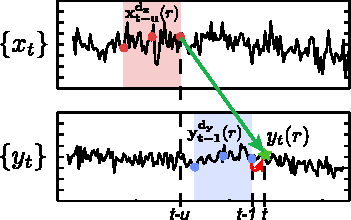
\includegraphics[scale=1.00]{figures/TE_concept.pdf}
	\caption[TE concept]{Transfer entropy (green arrow) between a source $\texttt{X}$ and a target process $\texttt{Y}$. Red and blue boxes indicate past states of both processes, the green star indicates the future value of $\textit{\texttt{Y}}$. $u$ indicates the interaction delay from $\texttt{X}$ to $\texttt{Y}$.}
	\label{fig:TE_concept}
\end{figure} 


\subsection{Notation and preliminaries}

\paragraph*{Notation} We assume, that TE is measured between two coupled physical systems $\mathcal{X}$ and $\mathcal{Y}$, that produce observable time series $\{x_1, \ldots, x_t, \ldots, x_N\}$ and $\{y_1, \ldots, y_t, \ldots, y_N\}$ with $t \in \{1 \ldots N\}$. We formalize these time series as realizations of random processes $\texttt{X}$, $\texttt{Y}$, which in turn are collections of random variables, $X_t$ and $Y_t$ (sorted by the integer $t$). Each random variable $X_t$, at a specific time $t$, has a set of $J$ possible outcomes $\mathcal{A}_{X_t} = \{a_1, \ldots, a_j, \ldots ,a_J \}$ , and their associated probability density function (PDF) $p_{X_t} (x_t = a_j)$.  

\paragraph*{State space reconstruction} As TE is defined between states of the processes $\texttt{X}$ and $\texttt{Y}$, we need to reconstruct these states from scalar observations $\{x_t\}$ and $\{y_t\}$. A state refers to a set of variables, that fully characterizes all relevant parameters to sufficiently describe a process at any given moment in time. The set of all possible states of a system is called the state space. TRENTOOL reconstructs states from scalar time series using time-delay embedding \cite{takens1981} under the assumption, that each process can be approximated by a Markov process. Time-delay embedding for an observation at time $t$ takes the form

\begin{equation}
  \mathbf{x}_t^{d_x}=\left( x_t,x_{t-\tau}, \ldots, x_{t-(d_x-1)\tau}\right),
\end{equation}

where $d_x$ is the embedding dimension and $\tau$ the embedding delay. TRENTOOL optimizes both parameters according to Ragwitz' criterion \cite{ragwitz2002}, where $d_x$ and $\tau$ are jointly optimized to minimize the prediction error of a local predictor, that predicts the future of each signal from its past.

\paragraph*{Stationarity} TE or other information theoretic functionals are calculated from the PDFs of the quantities involved. PDFs are typically not known \textit{a priori} and have to be estimated from multiple observed realizations of a random variable. How these realizations are obtained from data depends on whether the process in question is stationary or non-stationary. Stationarity of a process means that PDFs of the random variables that form the random process do not change over time, such that $p_{X_t}(x_t=a_j) = p_{X_{s}}(x_s=a_j),\  \forall s,t \in \mathbb{N}$. Any PDF $p_{X_t}(\cdot)$ may then be estimated from one observation of process $\mathtt{X}$ by means of collecting realizations $(x_1,\ldots, x_N)$ \emph{over time}. For processes that are non-stationary, i.e. $p_{X_t}(x_t=a_j) \neq p_{X_{s}}(x_s=a_j),\  \forall s,t \in \mathbb{N}$, temporal pooling is not applicable as PDFs vary over time $t$ and every random variable $X_t$ is associated with a different PDF $p_{X_t}(\cdot)$. 

TRENTOOL implements TE estimators for both stationary and non-stationary time series. The estimator assuming stationarity pools observations over time for PDF estimation. For non-stationary processes it is possible to repeat a process in time and pool observations over repetitions (see \citeA{gomez-herrero2010} and \citeA{wollstadt2013}). We call the repeated observations of a process an ensemble of time series. For an observation at time $t$ from a repetition $r = 1, \ldots, R$, we write $x_t(r)$. Note, that $t$ now refers to a time point $t$ relative to the onset $T$ of repetition $r$. If we choose the number of repetitions large enough, i.e. there is a sufficiently large set $\mathcal{R} = |R|$ of time points $T$, at which the process is repeated, we can assume that PDFs $p_{X_{T+t}}(\cdot)$ at time point $t$ relative to the onset of the repetition at $T$ are equal over all $R$ repetitions. We may obtain a reliable estimation of $p_{X_{T+t}}(\cdot)$ from this ensemble by evaluating $p_{\cdot}(\cdot)$ over 
all observations $x_{T+t},\forall T \in \mathcal{R}$. 


\subsection{Practical TE estimation in TRENTOOL}\label{sec:practical_TE}


\paragraph*{Transfer entropy functional} TRENTOOL allows for TE estimation from both stationary and non-stationary time series. We here present the TE functional $TE_{SPO}$ for TE estimation from an ensemble of time series \cite{lindner2011,vicente2011,wibral2013,wollstadt2013}. The $TE_{SPO}$ estimator allows for TE estimation from non-stationary ensemble data as well as for TE estimation from stationary time series as a special case: 

\begin{equation}
\label{eq:TE_u}
\begin{split}
TE_{SPO}\left(\textit{\texttt{X}}\rightarrow \textit{\texttt{Y}},t,u\right)= \sum_{\substack{y_{t}(r),\mathbf{y}^{d_{y}}_{t-1}(r),\mathbf{x}^{d_{x}}_{t-u}(r)\\ \in \mathcal{A}_{Y_t,\mathbf{Y}_{t-1}^{d_y},\mathbf{X}_{t-u}^{d_x}}}} p\left( y_{t}(r), \mathbf{y}^{d_{y}}_{t-1}(r), \mathbf{x}^{d_{x}}_{t-u}(r)  \right) \\ 
\log \frac{p\left( y_{t}(r) | \mathbf{y}^{d_{y}}_{t-1}(r), \mathbf{x}^{d_{x}}_{t-u}(r) \right)}
  {p\left(y_{t}(r) | \mathbf{y}^{d_{y}}_{t-1}(r)\right)} \, , 
\end{split}
\end{equation}

where $y_t(r)$ denotes the future observation of $\textit{\texttt{Y}}$ in repetition $r=1,\ldots,R$; $\mathbf{y}^{d_{y}}_{t-1}(r)$ denotes the past state of $\textit{\texttt{Y}}$ in repetition $r$ and $\mathbf{x}^{d_{x}}_{t-u}(r)$ denotes the past state of $\textit{\texttt{X}}$ in repetition $r$. $u$ is the delay of the information transfer between processes $\textit{\texttt{X}}$ and $\textit{\texttt{Y}}$ \cite{wibral2013}. In order to estimate the involved PDFs, necessary realizations of the respective random variables may be obtained through \textit{ensemble evaluation} over repetitions $r$ or through evaluation over time (for stationary time series). For a completely stationary time series, the estimator may be evaluated over one repetition and all available time points. For non-stationary time series, the estimator may be iteratively evaluated over all repetitions at each time point. Also, the estimator allows to combine both approaches by pooling observations over repetitions and over time windows for 
which local stationarity can be assumed. 


\paragraph*{Transfer entropy estimator} For practical TE estimation in TRENTOOL using equation \ref{eq:TE_u}, we proceed by first rewriting the estimator as a sum of four individual Shannon entropies:

\begin{equation}
\label{eq:TE_shannon}
\begin{split}
TE_{SPO}\left(\textit{\texttt{X}}\rightarrow \textit{\texttt{Y}},t,u\right) = H\left(\mathbf{Y}^{d_{Y}}_{t-1}, \mathbf{X}^{d_{X}}_{t-u}  \right) - H\left(Y_{t}, \mathbf{Y}^{d_{Y}}_{t-1}, \mathbf{X}^{d_{X}}_{t-u}  \right)\\
 + H\left( Y_{t}, \mathbf{Y}^{d_{Y}}_{t-1} \right) - H \left( \mathbf{Y}^{d_{Y}}_{t-1} \right) \,,
\end{split}
\end{equation}

The Shannon differential entropies $H$ can be efficiently estimated using nearest neighbor techniques \cite{kozachenko1987,victor2002}. TRENTOOL uses a modified Kraskov-St\"{o}gbauer-Grassberger estimator for transfer entropy \cite{kraskov2004}:

\begin{equation}
\label{eq:TE_kras}
\begin{split}
TE_{SPO}\left(\textit{\texttt{X}}\rightarrow \textit{\texttt{Y}},u,t_0,\Delta t\right) = \\ \psi\left(k\right)
  +\langle 
    \psi  \left( n_{\mathbf{y_{t-1}^{d_{y}}}(r)} +1 \right)\\
    -\psi \left( n_{y_t(r)\   \mathbf{y_{t-1}^{d_y}}(r)} +1 \right)\\
    -\psi \left( n_{\mathbf{y_{t-1}^{d_y}}(r)\   \mathbf{x_{t-u}^{d_x}}(r)} +1 \right) 
  \rangle_{r,t}, \\
  \forall r, t_0-\frac{\Delta}{2} \leq t \leq t_0 + \frac{\Delta}{2},
\end{split}
\end{equation}

% \begin{align}
% \label{eq:TE_kras}
% TE_{SPO}\left(\textit{\texttt{X}}\rightarrow \textit{\texttt{Y}},u,t_0,\Delta t\right) =& \\ &\psi\left(k\right) +\langle \psi  \left( n_{\mathbf{y_{t-1}^{d_{y}}}(r)} +1 \right)\\
%     &-\psi \left( n_{y_t(r)\   \mathbf{y_{t-1}^{d_y}}(r)} +1 \right)\\
%     &-\psi \left( n_{\mathbf{y_{t-1}^{d_y}}(r)\   \mathbf{x_{t-u}^{d_x}}(r)} +1 \right) 
%   \rangle_{r,t} \\
%   &\forall r, t_0-\frac{\Delta}{2} \leq t \leq t_0 + \frac{\Delta}{2}\, , 
% \end{align}

\noindent where $\psi$ denotes the digamma function and the angle brackets ($<\cdot>_r$) indicate an averaging over points in different repetitions $r$ in time window $t$ ($t\in[t^-;t^+]$ and $t^-\leq t \leq t^+$, where $\Delta t=t^+-t^-$). The distances to the $k$-th nearest neighbor in the highest dimensional space (spanned by $X_t, \mathbf{Y}^{d_{y}}_{t-1}, \mathbf{X}^{d_{x}}_{t-u}$) define the radius of the spheres for the counting of the number of points ($n_{\cdot}$) in these spheres around each state vector ($\cdot$) involved. 

Equation \ref{eq:TE_kras} is the most flexible formulation of the estimator implemented in TRENTOOL. It allows to obtain neighbor counts from pooling over time $t$ and/or pooling over repetitions $r$. We implemented two TE estimation strategies derived from this estimator. The first allows for mere temporal pooling (eq. \ref{eq:TE_kras_t}, estimating TE for each repetition $r$ separately, see section \ref{sec:core_functions}, \textit{TRENTOOL core functions}). The second allows for mere ensemble pooling (eq. \ref{eq:TE_kras_r}) or a combination of ensemble and temporal pooling (eq. \ref{eq:TE_kras}, see section \ref{sec:ensemble_method}, \textit{Estimating time-resolved transfer entropy}). 

\begin{equation}
\label{eq:TE_kras_t}
\begin{split}
TE_{SPO}\left(\textit{\texttt{X}}\rightarrow \textit{\texttt{Y}},u,r_i\right) = &\psi\left(k\right) +\langle \psi  \left( n_{\mathbf{y_{t-1}^{d_{y}}}(r_i)} +1 \right)\\
    &-\psi \left( n_{y_t(r_i)\   \mathbf{y_{t-1}^{d_y}}(r_i)} +1 \right)\\
    &-\psi \left( n_{\mathbf{y_{t-1}^{d_y}}(r_i)\   \mathbf{x_{t-u}^{d_x}}(r_i)} +1 \right)    
  \rangle_{t}, \, \forall t,
\end{split}
\end{equation}

\begin{equation}
\label{eq:TE_kras_r}
\begin{split}
TE_{SPO}\left(\textit{\texttt{X}}\rightarrow \textit{\texttt{Y}},u,t\right) = \psi\left(k\right)
  +\langle 
    \psi  \left( n_{\mathbf{y_{t-1}^{d_{y}}}(r)} +1 \right)\\
    -\psi \left( n_{y_t(r)\   \mathbf{y_{t-1}^{d_y}}(r)} +1 \right)\\
    -\psi \left( n_{\mathbf{y_{t-1}^{d_y}}(r)\   \mathbf{x_{t-u}^{d_x}}(r)} +1 \right) 
  \rangle_{r}, \, \forall r,
\end{split}
\end{equation}


\paragraph*{TRENTOOL analysis steps} TRENTOOL uses the estimator in equations \ref{eq:TE_kras} for TE estimation. To estimate TE from scalar time series using the estimators, TRENTOOL proceeds as follows:

\begin{enumerate}
 \item Parameters for state space reconstruction are optimized for a given pair of time series according to Ragwitz' criterion \cite{ragwitz2002}
 \item Time series are embedded using optimized parameters
 \item Embedded time series are pooled over time and/or repetitions to form a state space for nearest neighbor searching 
 \item State spaces are searched using nearest neighbor techniques \cite{kraskov2004}
 \item Nearest neighbor counts resulting from nearest neighbor searches are used for TE calculation according to eq. \ref{eq:TE_kras}
 \item Resulting TE values are tested for statistical significance using non-parametric permutation testing to account for the bias introduced by the estimator \cite{lindner2011,vicente2011}
 \item Test for volume conduction using a shift test \cite{lindner2011} or additional conditioning \cite{faes2013}
\end{enumerate}

This is the core functionality for TE estimation in TRENTOOL. The practical use of TE estimation in TRENTOOL is described in more detail in section \ref{sec:core_functions}, \textit{TRENTOOL core functions}. Additional functionalities provided by the toolbox are described in the next subsection.

\subsection{Additional functionalities implemented in TRENTOOL} \label{sec:additional_functionalities}

TRENTOOL provides additional functionalities for TE estimation and statistical testing, especially for TE estimation from neural data:

\begin{itemize}
 \item Reconstruction of interaction delays \cite{wibral2013}
 \item Estimation of time-resolved TE from an ensemble of time series \cite{wollstadt2013,gomez-herrero2010}
 \item Group analysis and statistical testing \cite{lindner2011}
 \item Graph algorithm for partial correction for multivariate interactions between more than two analyzed time series \cite{wibralIEEE}
\end{itemize}

Background information on the presented functionalities can be found in the respective articles. The following subsections provide short introductions to each functionality to enable the user to chose the appropriate analysis steps for a given data set.

\subsubsection{Reconstruction of interaction delays}

We recently showed, that the TE functional implemented in TRENTOOL (eq. \ref{eq:TE_u}) allows for the reconstruction of interaction delays between the two analyzed processes \cite{wibral2013}. We showed that the estimated TE value becomes maximal when the parameter $u$ is equal to the true interaction delay $\delta$. Thus, our estimator may be used to recover $\delta$ from a set of assumed candidate values $u$:

\begin{equation}
  \label{eq:delta_max}
  \delta = arg\,\operatorname*{max}_u \  TE_{SPO}(X \rightarrow Y,u)
\end{equation}

This functionality is implemented in TRENTOOL by looping over TRENTOOL's core functions using varying values for $u$. Using TRENTOOL for interaction delay reconstruction is described in more detail in section \ref{sec:interaction_delays}, \textit{Reconstruction of interaction delays}.


\subsubsection{Estimating TE from an ensemble of time series}

Gomez-Herrero and colleagues showed that it is possible to estimate the necessary probability density functions for TE calculation from an ensemble of time series \cite{gomez-herrero2010}. We implemented the ensemble method for TE estimation in TRENTOOL, allowing the treatment of non-stationary time series and the estimation of time-resolved TE \cite{wollstadt2013}. Using this ensemble method circumvents the necessity of temporal pooling by using ensemble pooling over repeated observations. The use of the ensemble method is described in more detail in section \ref{sec:ensemble_method}, \textit{Estimating time-resolved transfer entropy from an ensemble of time series}.

\subsubsection{Group analysis}

TRENTOOL allows for the statistical comparison of TE values between two sets of data (e.g. two conditions or subject groups in an experiment) \cite{lindner2011}. TRENTOOL choses common estimation parameters over all data sets to be analyzed, which are then used in individual TE estimation. Using common parameters for TE estimation allows for a statistical comparison of estimated TE values between groups, because statistical differences can be attributed to differences in information transfer rather than differences in the estimation parameters. Group differences are tested using a non-parametric permutation test \cite{maris2007,lindner2011}. The use of the group analysis is described in more detail in section \ref{sec:groupanalysis}, \textit{Group analysis in TRENTOOL}.

\subsubsection{Graph correction for multivariate effects}

TRENTOOL estimates TE between \textit{pairs} of processes. However, if a system consists of more than two processes, multivariate interactions between these processes may take place. If multivariate interactions occur, the iterative analysis of pairs of processes, i.e. bivariate analysis, may return spurious information transfer \cite{kaminski2001,blinowska2004,lizier2013}. Spurious information transfer may result from one of two interaction schemes: cascade effects or common drive (Figure \ref{fig:spurious_effects}). TRENTOOL allows for a partial post-hoc correction of these spurious results using a graph-based algorithm on the network of information transfer in a multivariate system \cite{wibralIEEE}. This post-hoc correction may be used on any information transfer network resulting from \textit{neural data} as it uses assumption valid for neural systems only. The use of the post-hoc correction is described in more detail in section \ref{sec:graphanalysis}, \textit{Graph correction for cascade effects and 
simple common drive}.

\begin{figure}[H]	
	\centering
 		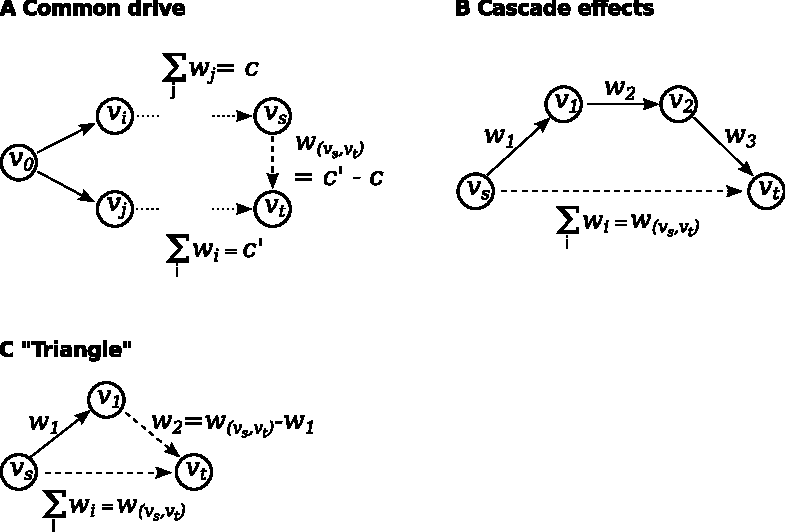
\includegraphics[scale=0.85]{figures/spurious_effects.pdf}
	\caption[Spurious results]{Network coupling schemes, that may lead to the detection of spurious information transfer. 
	\textbf{A} Common drive: Processes $v_s$ and $v_t$ are driven by process $v_0$ with summed delays $c$ and $c'$ respectively. Bivariate analysis may detect a spurious information transfer between $v_s$ and $v_t$. 
	\textbf{B} Cascade effect: Information is transferred from $v_s$ to $v_t$ via nodes $v_1$ and $v_2$. Bivariate analysis may detect a spurious direct information transfer between $v_s$ and $v_t$.
	\textbf{C} ``Triangle'': In a bivariately analyzed triangle, cascade effects ($v_s\stackrel{w_{(v_s,v_t)}}{\rightarrow}v_t$) and common drive effect ($v_1\stackrel{w_{(v_1,v_t)}}{\rightarrow}v_t$) will not be distinguishable.}
	\label{fig:spurious_effects}
\end{figure}







\newpage
\section{Using TRENTOOL} \label{sec:using_TRENTOOL}

\subsection{Overview} \label{sec:overview}

% TODO ask Michael if this okay like this
\paragraph*{Analysis strategies} TRENTOOL provides core functions for TE estimation as described in section \ref{sec:practical_TE}. These core functions may be combined with the additional functionalities presented in section \ref{sec:additional_functionalities}. Whether functionalities are applicable to a given set of data depends on the experimental design. %Figure \ref{fig:analysis_strategy} provide an overview over intended analysis strategies and the according requirements for the data. % TODO fix this

All TRENTOOL functionalities are accessible via calls to the respective MATLAB functions and may be combined into \textit{analysis scripts}. Examples for analysis scripts for different analysis strategies can be found in section \ref{sec:example_scripts}. 

% % TODO make a figure, include references to functions and sections in this manual
% \begin{figure}[H]	
% 	\centering
%  		\includegraphics[scale=0.85]{figures/analysis_strategy.pdf}
% 	\caption[Analysis Strategies]{Analysis strategies for data from different experimental designs.
% 	\textbf{A} Single Subject Analysis: Data are analyzed for individual subjects and tested against surrogate data. This results in a network of significant information flow for each subject. Single subject analysis may either be conducted by pooling data over time (\textbf{a}) or by using the ensemble method (\textbf{b}) to obtain a time-resolved estimation of information transfer. Whether a link occurred a statistical significant number of times over single subjects may be tested using a binomial test (\textbf{c}).
% 	\textbf{B} Group Analysis for two sets of data: Data are analyzed using common embedding parameters for all subjects; results are then tested for differences between both sets of data. This analysis strategy for the quantitative comparison of TE between two groups of data (e.g. between data recorded in two conditions or between two groups of participants. TE estimation may either be conducted by pooling data over time (\textbf{a}) or by using the ensemble method (\textbf{b}) to obtain a time-resolved estimation of information transfer.
% 	}
% 	\label{fig:analysis_strategy}
% \end{figure}

%TRENTOOL provides a core work flow for TE estimation according to section \ref{sec:practical_TE} as well as additional functionalities presented in section  \ref{sec:additional_functionalities}. All these functionalities are provided as MATLAB functions (see Figure \ref{fig:TRENTOOL3_workflow_overview} for an overview). Users may combine these functions into an \textit{analysis script} that is appropriate for their data. Figure \ref{fig:analysis_strategy} provides an overview of analysis strategies for different experimental designs. In every analysis, TRENTOOL's core functions are used for TE estimation following the approach presented in the \textit{Background} section.

\paragraph*{TRENTOOL core functions} TRENTOOL's core functions for TE estimation provide all necessary functionalities to estimate TE from a set of time series. The core functions implement two main analysis steps (Figure \ref{fig:core_functions}):

\begin{enumerate}
 \item data preparation (optimization of embedding parameters)
 \item TE estimation from prepared data (data embedding using optimized parameters and TE calculation from nearest neighbor statistics)
\end{enumerate}

Depending on the user's analysis script, the user calls functions for data preparation and TE estimation directly (Figure \ref{fig:TRENTOOL3_workflow_overview}, panel A and B) or calls wrapper functions, that encapsulate both analysis steps and provide additional functionality (Figure \ref{fig:TRENTOOL3_workflow_overview}, panel C and D). In general we recommend the use of the work flow for interaction delay reconstruction presented in section \ref{sec:interaction_delays}. This work flow may be used both for single subject analysis (TE estimation for individual subjects or conditions) as well as for group statistics (comparison of TE values between two sets of data, see section \ref{sec:groupanalysis}).

\paragraph*{Organization of the following subsections} We will first present TRENTOOL's core functions for data preparation and TE estimation for a single set of times series (e.g. a single subject measured in one experimental condition). We will then present analysis strategies building on the core functions in section \ref{sec:additional_functionalities}. Example analysis scripts are provided in section \ref{sec:example_scripts}, \textit{Example Scripts}.

The following subsections are structured as follows: Each subsection describes one TRENTOOL analysis strategy. For each strategy, we first give a brief overview of the implementation of the pipeline, followed by detailed descriptions of the functions, users interact with. Detailed descriptions of input and output parameters are given in table form in section \ref{sec:appendix}, \textit{Appendix}.

\paragraph*{Input data} The main input to TRENTOOL consists of data to be processed and additional function parameters that specify how the data are processed. Data may be passed to TRENTOOL as a structure in the FieldTrip raw data format (table \ref{tab:input_data}, see also \cite{oostenveld2011} and \url{http://fieldtrip.fcdonders.nl/}). Function parameters are passed within a MATLAB structure, following the general FieldTrip coding convention. Throughout this documentation, we will refer to these parameter structures as \verb&cfgXXX&, where \verb&XXX& is replaced by an abbreviation for the function that is called with the cfg structure in question.


\begin{table}[H]
\small
\caption[Input data]{Input data in TRENTOOL: Fields in a FieldTrip raw data structure (TRENTOOL Version 3.3)} 
\begin{tabular}{p{2cm}p{2.5cm}p{2.5cm}p{1.1cm}p{5.5cm}} \toprule
\textbf{field name} & \textbf{dimension} & \textbf{data type} & \textbf{units} & \textbf{description} \\ \midrule
\verb+trial+ & \{no. trials\}[no. channels x no. samples] & cell array of double arrays & & data for each trial, where each trial holds samples from all channels\\
\rowcolor{Gray}
\verb+time+ & \{no. trials\}[1 x no. samples] & cell array of double arrays  & seconds & time indices for individual trials\\
\verb+label+ & \{no. channels x 1\} & cell of strings & & labels of channels\\
\bottomrule
\label{tab:input_data}
\end{tabular}
\end{table}

\begin{figure}[H]	
	\centering 	
 		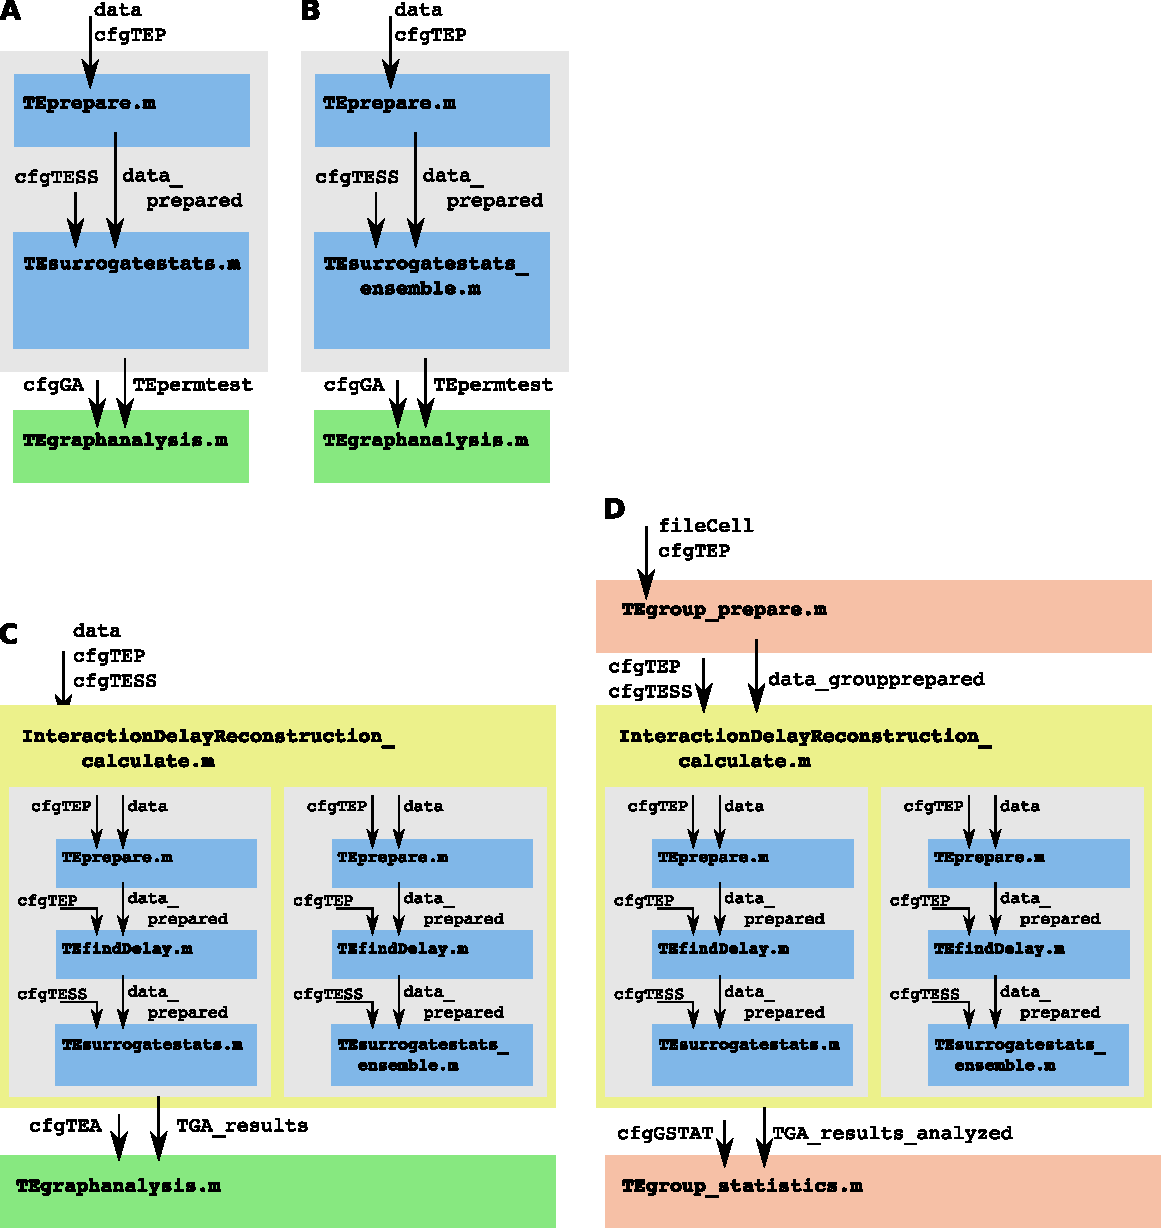
\includegraphics[width=0.85\textwidth]{figures/TRENTOOL3_workflow_main.pdf}
	\caption[Overview TRENTOOL functions]{Overview of TRENTOOL functions: 
	(A) TRENTOOL core functions for TE estimation (sec. \ref{sec:core_functions}); 
	(B) TRENTOOL core functions for TE estimation using the ensemble method (sec. \ref{sec:ensemble_method}); 
	(C) Reconstruction of interaction delays (sec. \ref{sec:interaction_delays}): The function \texttt{InteractionDelayReconstruction\_calculate.m} calls functions \texttt{TEprepare.m}, \texttt{TEfindDelay.m}, and \texttt{TEsurrogatestats.m} or \texttt{TEsurrogatestats\_ensemble.m} to prepare the data, reconstruct interaction delays and perform surrogate statistics on estimated TE values.
	(D) Group analysis (sec. \ref{sec:groupanalysis}: The function \texttt{TEgroup\_prepare.m} prepares data sets for group analysis, TE is estimated using the functionality presented in (C), function \texttt{TEgroup\_stats.m} tests TE values for significant differences;
	(A-C) TE estimates may be partially corrected for spurious information flow due to multivariate interactions using a graph algorithm (\texttt{TEgraphanalysis.m}, green boxes, see section \ref{sec:graphanalysis}).}
	\label{fig:TRENTOOL3_workflow_overview}
\end{figure}


\subsection{TRENTOOL core functions}\label{sec:core_functions}

The TRENTOOL core functions realize the two analysis steps of data preparation and TE estimation from prepared data (Fig. \ref{fig:core_functions}). The functions comprise of \verb&TEprepare.m& for data preparation and \verb&TEsurrogatestats& for TE estimation from prepared data (following the approach lined out in section \ref{sec:background}, \textit{Background}). Note that TRENTOOL analyses \textit{pairs} of signals only, i.e. TRENTOOL does not estimate multivariate TE from a set of time series, but estimates TE for pairs of time series iteratively (pairs of time series have to be defined by the user, see next subsection).


\begin{figure}[H]	
	\centering 
 		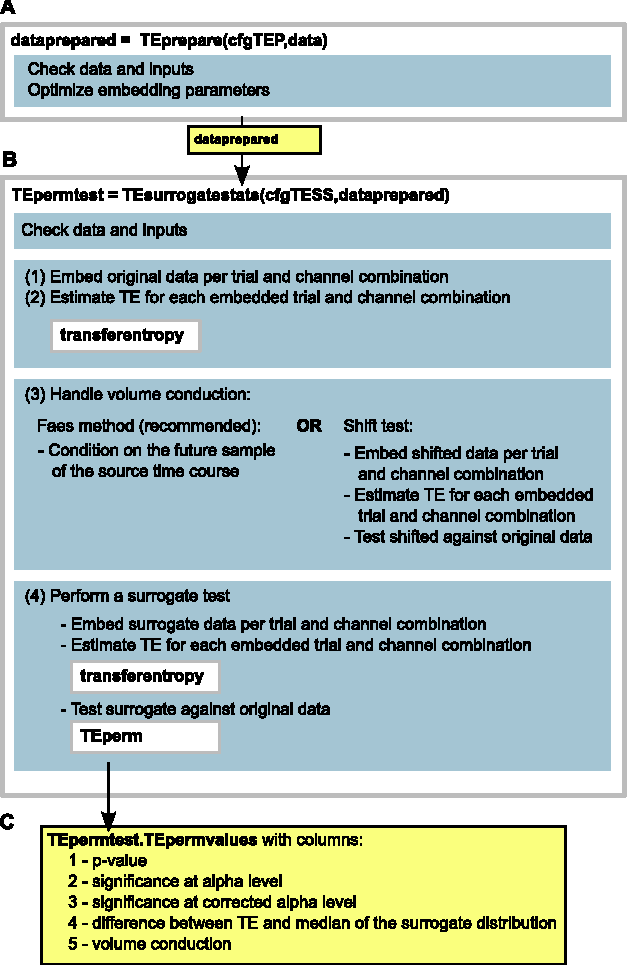
\includegraphics[width=0.60\textwidth]{figures/TRENTOOL3_workflow_CPU.pdf}
	\caption[TRENTOOL core functions]{TRENTOOL core functions. (A) Data preparation and optimization of embedding parameters using \texttt{TEprepare.m}; (B) TE estimation and statistical testing from prepared data: (1) Embedding of original data and (2) TE estimation per trial and channel combination, (3) optional shift test (defined in \texttt{cfgTESS.shifttest}), (4) test against surrogate data using trial shuffling; (C) Output structure \texttt{TEpermtest}, containing the field \texttt{.TEpermvalues} holding TE results for each channel combination (see table \ref{tab:TEpermtest}).}
	\label{fig:core_functions}
\end{figure}


\subsubsection{\texttt{TEprepare.m}} \label{sec:TEprepare}

\paragraph*{Description} \verb&TEprepare.m& checks the input provided by the user and optimizes the embedding dimension $d$ and embedding delay $\tau$ for subsequent TE estimation using Ragwitz' criterion (\cite{ragwitz2002}). 

\paragraph*{Usage} \verb&data_prepared = TEprepare(cfgTEP,data);&

\paragraph*{Input} \texttt{data} contains data in the FieldTrip raw data format (table \ref{tab:input_data}), \verb&cfgTEP& contains a configuration structure with analysis parameters (table \ref{tab:cfgTEP}).

\verb&cfgTEP& has to contain information regarding the combinations of signals the user wishes to analyze. Signal combinations can be defined by the user as a $2$ by $n$ cell array of strings, that contains $n$ pairs of signal labels (\texttt{cfgTEP.sgncmb}). Alternatively, the user can provide a cell array of strings, that contains a list of signal labels from which TRENTOOL constructs all pairs of signal combinations (\texttt{cfgTEP.channel}).

%\texttt{TEprepare} requires the path to the TSTOOL toolbox (\texttt{cfg.Path2TSTOOL}).

If the user wants to use the ensemble method for TE analysis (see section \ref{sec:ensemble_method}), the field \texttt{cfgTEP.ensemblemethod} has to be set to \texttt{'yes'}. Parameters for TE estimation (\texttt{cfgTESS}) have to be changed accordingly (see next subsection and table \ref{tab:cfgTESS}).

\paragraph*{Output} Results (optimized embedding parameters, parameters for TE estimation) are appended to the data structure as a separate field \verb&.TEprepare& (table \ref{tab:TEprepare}). The resulting data structure \texttt{data\_prepared} may be used as input to \texttt{TEsurrogatestats.m} or \texttt{TEsurrogatestats\_ensemble.m} for TE estimation (see below).


\subsubsection{\texttt{TEsurrogatestats.m}} \label{sec:TEsurrogatestats}

\paragraph*{Description} \verb&TEsurrogatestats.m& estimates TE from the prepared data returned by \texttt{TEpre-\\pare.m}, using the optimized embedding parameters. \texttt{TEsurrogatestats} performs the following analysis steps on the data: 

\begin{itemize}
 \item Check input data and parameters
 \item Estimate TE for original data:
 \begin{itemize}
  \item Embed individual trials using optimized parameters
  \item Perform nearest neighbor searches on reconstructed state spaces
  \item Calculate TE from neighbor counts
 \end{itemize}
 \item Optional: Perform a shift test or use extra conditioning to handle volume conduction (see below)
 \item Estimate TE for surrogate data (analogous to original data)
 \item Perform a statistical test of TE values from original data against surrogate TE values
 \item Save results
\end{itemize}

\paragraph*{Usage} \verb&TEpermtest = TEsurrogatestats(cfgTESS,data_prepared);&

\paragraph*{Input} \texttt{data\_prepared} contains data prepared by \verb&TEprepare.m&, \verb&cfgTESS& contains a configuration structure with analysis parameters (table \ref{tab:cfgTESS}).

It is recommended to use the embedding parameters optimized by \texttt{TEprepare.m} (see section \ref{sec:TEprepare}) and not set \texttt{cfgTESS.dim} and \texttt{cfgTESS.tau} manually (see table \ref{tab:cfgTESS}). 

The user may chose to perform a shift test on the data (\texttt{cfgTESS.shifttest = 'yes'}), to test for volume conduction in the data \cite{lindner2011}. Alternatively, the user may use an extra conditioning (\texttt{cfgTESS.extracond = 'Faes\_Method'}) \cite{faes2013}, which includes the future sample of the source at the prediction time into the state vector of the past of of the target to condition on it (such that $TE = I\left(y^+;\mathbf{x}^-|\mathbf{y}^-; x^+\right)$). In principle, this removes any volume conduction effect and makes the conduction of a shift test unnecessary, thus the shift test and Faes Method are mutually exclusive. We recommend the use of extra conditioning over the shift test.
%\verb+Battaglia_Method+: This methods conditions on the "mean activity" of the system, i.e. a global system state.This will be done by creating a channel carrying that signal which will then be used as an additional entry for the past state of the source

For the creation of surrogate data for statistical testing (\verb+cfgTEP.surrogatetype+) one of the following strategies may be chosen \cite{lindner2011}:

\begin{table}[H]
\begin{tabularx}{\textwidth}{lL{5cm}X} \toprule
\textbf{Parameter} & \textbf{Strategy} & \textbf{Example} \\
		   & 		       & (original: 1 2 3 4 5 6) \\ \midrule
\texttt{trialshuffling} &  trial(n+1) & 2 3 4 5 6 1 \\
\texttt{trialreverse}   &  reverse of trial(n) & 6 5 4 3 2 1 \\
\texttt{blockresampling} & cuts trial(n) at random point and resamples the trial &4 5 6 1 2 3 \\
\texttt{blockreverse1}   & reverse after blockresampling & 3 2 1 6 5 4 \\
\texttt{blockreverse2}   & reverse first block after blockresampling & 6 5 4 1 2 3\\
\texttt{blockreverse3}   & reverse second block after blockresampling & 4 5 6 3 2 1 \\
\texttt{swapneighbors}   & pair odd trials with the higher neighbor and 3even with the lower neighbor & 2 1 4 3 6 5\\ \bottomrule
\end{tabularx} \label{tab:surrogatetype}
\end{table}


\paragraph*{Output} The results of TE estimation and statistical testing are returned to the user as a structure \texttt{TEpermtest} (see table \ref{tab:TEpermtest}). This structure contains the results of the statistical testing and is also save to disk as \texttt{*\_TEpermtest\_output.mat'}, using the string in \texttt{cfgTESS.fileidout} as prefix. Additionally, raw TE values are saved to disk (structure \texttt{TEresult}, table \ref{tab:TEresult}) as \texttt{*\_TE\_output.mat'}, again using \texttt{cfgTESS.fileidout} as prefix.


\subsection{Reconstruction of interaction delays} \label{sec:interaction_delays}

TRENTOOL allows for the reconstruction of interaction delays between time series by scanning over assumed interaction delays $u$ \cite{wibral2013}. The true interaction delay may be estimated by finding the maximum TE value over all scanned interaction delays. This functionality is provided within the function \verb&InteractionDelayReconstruction_calculate.m& (Figure \ref{fig:workflow_delayReconstruction}): The function estimates TE for each channel combination and assumed delay $u$ using the TRENTOOL core functions (section \ref{sec:core_functions}). Estimated TE values are passed to the function \verb&InteractionDelayReconstruction_analyze.m&, that finds the maximum TE value over all $u$ for each channel combination (eq. \ref{eq:delta_max}). TE values at this interaction delay are then tested for statistical significance using the functions \verb&TEsurrogatestats.m& or \verb&TEsurrogatestats_ensemble.m& (section \ref{sec:ensemble_method}, \textit{Estimating time-resolved transfer entropy from an ensemble of time series}). 

The approach for interaction delay reconstruction may also be used together with group analysis functionalities (section \ref{sec:groupanalysis}, \textit{Group analysis in TRENTOOL}). For an example analysis, see example scripts \ref{lst:delayreconstruction_CPU} and \ref{lst:delayreconstruction_GPU}. 

Note: Using the functions \verb&InteractionDelayReconstruction_*& is the recommended analysis strategy for most neural data sets.

\begin{figure}[H]	
	\centering	
 		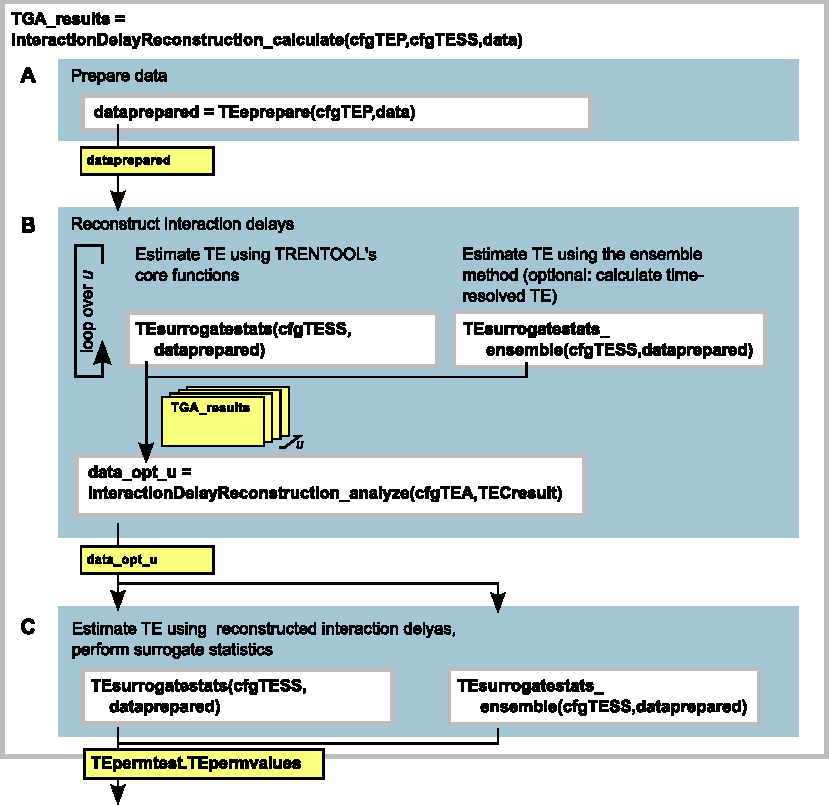
\includegraphics[scale=0.90]{figures/TRENTOOL3_workflow_delayreconstruction.pdf}
	\caption[TRENTOOL work flow for interaction delay reconstruction]{TRENTOOL work flow for interaction delay reconstruction. The function \texttt{InteractionDelayReconstruction\_calculate} first calls \texttt{TEprepare} on the input data (A). Prepared data is then passed to \texttt{TEfindDelay} (B) to reconstruct the optimal interaction delay by looping over TE estimation using varying values for $u$. TE may be estimated using \texttt{TEsurrogatestats} (see section \ref{sec:core_functions}) or \texttt{TEsurrogatestats\_ensemble} (see section \ref{sec:ensemble_method}), while using \texttt{TEsurrogatestats\_ensemble} allows the user to additionally calculate time-resolved TE. The function \texttt{TEfindmaxte} finds the $u$ that maximizes TE and adds this $u_{opt}$ to every channel combination in the \texttt{dataprepared} structure. In a third step (C) final TE values are estimated from \texttt{dataprepared}, using the reconstructed interaction delays and a statistical test is performed.	
	}
	\label{fig:workflow_delayReconstruction}
\end{figure} 

\subsubsection{\texttt{InteractionDelayReconstruction\_calculate.m}} 

\paragraph*{Description} Wrapper function that estimates TE using optimized values for the interaction delay(see eq. \ref{eq:TE_u}). The function (1) prepares the data (calls \verb&TEprepare.m&); (2) optimizes interaction delays by estimating TE for all assumed values $u$ and finding the value $u$ that maximizes TE; (3) performes a statistical test on TE values estimated using the optimized interaction delay Figure \ref{fig:workflow_delayReconstruction}). TE values are estimated by the functions \verb&TEsurrogatestats.m& (see also section \ref{sec:core_functions}) or \verb&TEsurrogatestats_ensemble.m& (see also section \ref{sec:ensemble_method}).

\paragraph*{Usage} \texttt{TGA\_results = InteractionDelayReconstruction\_calculate(cfgTEP,cfgTESS,\\data);}

\paragraph*{Input} \texttt{data} contains input data in the FieldTrip raw data format (see section \ref{sec:overview} and table \ref{tab:input_data}), \verb&cfgTEP& (table \ref{tab:cfgTEP}) and \verb&cfgTESS& (table \ref{tab:cfgTESS}) contain configuration structures with analysis parameters for functions \verb&TEprepare.m& and \verb&TEsurrogatestats.m&, that are called inside the function.

\paragraph*{Output} The interaction delay and the associated statistics are returned as a structure \texttt{TEperm-\\test} similar to the structure returned by \verb&TEsurrogatestats.m& (table \ref{tab:TEpermtest}). Additionally, the table in the field \verb&.TEpermvalues& contains a sixth column that provides the optimal $u$ for each channel combination. Final results (output \texttt{TEpermtest}) are saved to disk using the string in \texttt{cfgTESS.fileidout} as prefix. These results may be visualized using the function \verb&InteractionDelayReconstruction\_plotting& (see next subsection).

\subsubsection{\texttt{InteractionDelayReconstruction\_plotting.m}} 

\paragraph*{Description} Function plots final results from TE analysis with \verb&InteractionDelayReconstruction_calculate.m&. The function plots TE values against assumed delays $u$ for each channel combination in the data set. 

\paragraph*{Usage} \texttt{InteractionDelayReconstruction\_plotting(cfgUPLOT, TEpermtest);}

\paragraph*{Input} \texttt{cfgUPLOT} (table \ref{tab:cfgUPLOT}) contains a configuration structure with plotting options. \texttt{TEpermtest} is the output of \texttt{InteractionDelayReconstruction\_calculate.m}.

\paragraph*{Output} The function plots normalized TE values ($TE/TE_{max}$) for each channel combination against assumed interaction delays u. 

%The function collects outputs \texttt{TEpermvalues} (table \ref{tab:TEpermtest}) from individual calls to \texttt{TEsur-\\rogatestats.m} (\verb&TEsurrogatestats_ensemble.m& respectively) and returns these in a cell array \verb&TGA_results& for further analysis by \verb&InteractionDelayReconstruction_analyze.m& (see next subsection). With each call to \verb&TEsurrogatestats.m& (\verb&TEsurrogatestats_ensemble.m& respectively), i.e. for each assumed interaction delay $u$, outputs \texttt{TEpermvalues} and \texttt{TEresult} are saved to disk using the string in \texttt{cfgTESS.fileidout} as prefix.

% \subsubsection{\texttt{InteractionDelayReconstruction\_analyze.m}}
% 
% \paragraph*{Description} The function finds the optimal $u$ for each analyzed channel combination, by finding the $u$ for which the estimated TE value becomes maximal (eq. \ref{eq:delta_max}). For each channel combination, all TE values and their respective p-value are compared over all values of $u$. The value of $u$ for which TE is a maximum is kept as the true interaction delay $\delta$.
% 
% \paragraph*{Usage} \verb&TGA_results_analyzed = InteractionDelayReconstruction_analyze(cfgTEA,TGA_results);&
% 
% \paragraph*{Input} \texttt{TGA\_results} contains individually analyzed data returned by \texttt{InteractionDelayRecon-\\struction\_calculate.m}, \texttt{cfgTEA} contains a configuration structure with analysis parameters (table \ref{tab:cfgTEA}).
% 
% \paragraph*{Output} The interaction delay and the associated statistics are returned as a structure \texttt{TEperm-\\test} similar to the structure returned by \verb&TEsurrogatestats.m& (table \ref{tab:TEpermtest}). Additionally, the table in the field \verb&.TEpermvalues& contains a sixth column that provides the optimal $u$ for each channel combination.


\subsection{Estimating time-resolved transfer entropy from an ensemble of time series}\label{sec:ensemble_method}

TRENTOOL allows for the estimation of TE from an ensemble of time series (see \cite{wollstadt2013} and \cite{gomez-herrero2010}). By using this ensemble approach, TRENTOOL allows for the estimation of TE from non-stationary processes and furthermore enables TE estimation in a time-resolved fashion. The ensemble approach is computationally demanding, thus TRENTOOL requires the use of a graphics processing unit (GPU) to speed up TE estimation when using the ensemble approach. 

% TODO future versions could include a figure, that makes time-resolved TE estimation more clear
TRENTOOL realizes the time-resolved estimation of TE by using user-defined analysis windows. Analysis windows can be defined by looping over calls to \texttt{TEprepare.m} and \texttt{TEsurrogatestats\_ensemble.m} with varying times of interests specified in \texttt{cfgTEP.toi}  (see example script \ref{lst:delayreconstruction_CPU}). Furthermore, time-resolved TE estimation may be combined with the reconstruction of interaction delays (see below) and group statistics functionalities (see sections \ref{sec:groupanalysis}, \textit{Group analysis in TRENTOOL}). For both analysis strategies, the user has to loop over calls to \texttt{InteractionDelayReconstruction\_calculate.m} using varying analysis windows specified in \texttt{cfgTEP.toi} to estimate time-resolved TE (example script \ref{lst:delayreconstruction_GPU}).

Using the ensemble method in TRENTOOL is similar to the usage of TRENTOOL's core functions (section \textit{TRENTOOL core functions}), with the exception that TE estimation is handled by the function \texttt{TEsurrogatestats\_ensemble.m} instead of \texttt{TEsurrogatestats.m}. Here, we will present the usage of \texttt{TEsurrogatestats\_ensemble.m} only as the use of \texttt{TEprepare.m} for data preparation prior to TE estimation remains the same as described in section \ref{sec:core_functions}. For an example analysis, see \ref{lst:delayreconstruction_GPU}.

\begin{figure}[H]	
	\centering 
 		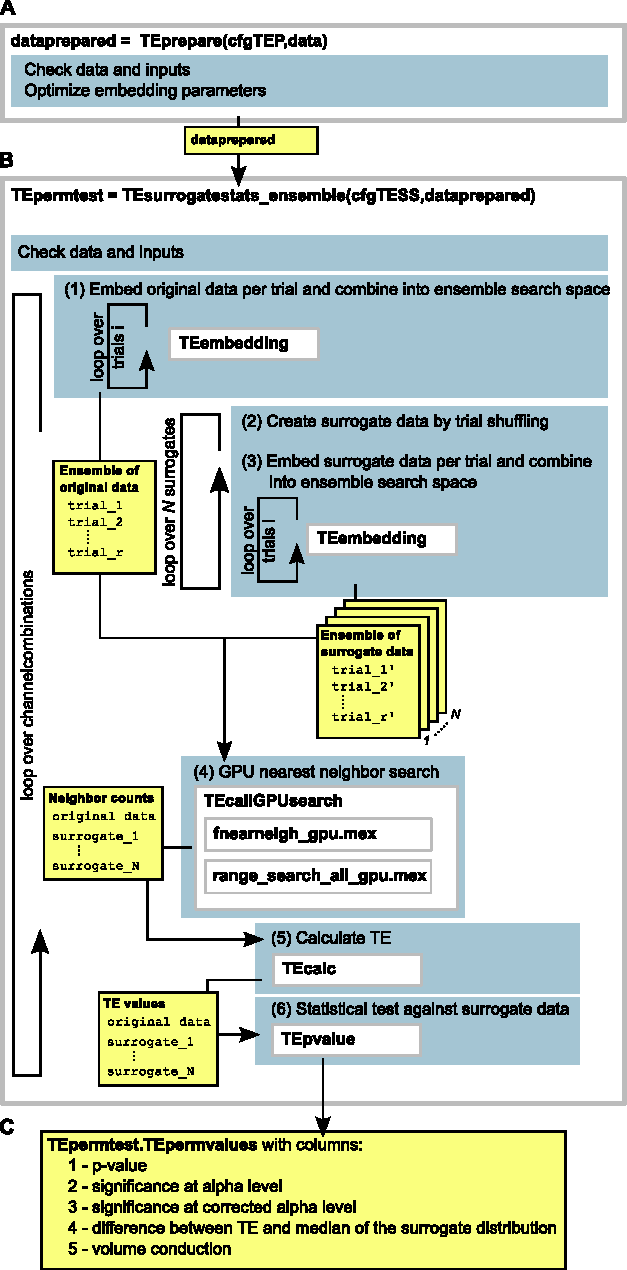
\includegraphics[scale=0.70]{figures/TRENTOOL3_workflow_ensemble.pdf}
	\caption[TRENTOOL Work flow ensemble method on GPU]{Using the ensemble method in TRENTOOL. 
	(A) Data preparation and optimization of embedding parameters using \texttt{TEprepare.m};
	(B) TE Estimation using a GPU for nearest neighbor searches;
	(C) Output structure \texttt{TEpermtest} containing the field \texttt{.TEpermvalues} holding TE results for each channel combination (see table \ref{tab:TEpermtest}).
	}
	\label{fig:workflow_ensemble}
\end{figure}

\subsubsection{\texttt{TEsurrogatestats\_ensemble.m}}

\paragraph*{Description} The function estimates TE from the prepared data returned by \verb&TEprepare.m&, using the optimized embedding parameters. The function estimates TE in six steps (Figure \ref{fig:workflow_ensemble}): 
\begin{enumerate}
  \item original data is embedded per repetition and repetitions are
concatenated forming the ensemble search space
  \item $N$ sets of surrogate data are created from the original
data by shuffling the repetitions of the target time series, 
  \item each surrogate dataset is embedded per repetition and concatenated forming one ensemble search space 
  \item all embedded original and surrogate data ensembles are concatenated and passed to a wrapper function that calls the GPU search functions to perform neighbor counts in parallel for each ensemble 
  \item TE values are calculated for original and surrogate data from the ensemble neighbor counts using the KSG-estimator \cite{kraskov2004}, 
  \item TE values for original data are tested statistically against the distribution of surrogate TE values.
\end{enumerate}

\paragraph*{Usage} \verb&TEpermtest = TEsurrogatestats_ensemble(cfgTESS,data_prepared);& 

\paragraph*{Input} \texttt{data\_prepared} contains data prepared by \verb&TEprepare.m&, \verb&cfgTESS& contains a configuration structure with analysis parameters (table \ref{tab:cfgTESS}). Note, that the use of the GPU has to be specified in the field \texttt{cfgTEP.ensemblemethod}, when calling \texttt{TEprepare.m} for data preparation. Additionally, the GPU's hardware parameters have to be provided to \texttt{TEsurrogatestats\_ensemble.m} (\verb+cfgTESS.GPUmemsize+, \verb+cfgTESS.numthreads+, \verb+cfgTESS.maxgriddim+). 

When using the ensemble method, the use of the Faes-Method is mandatory (\texttt{cfgTESS.extracond = 'Faes\_Method'}) and the shift test has to be switched off (\texttt{cfgTESS.shifttest = 'no';}). The use of the Faes method prevents the detection of information transfer due to volume conduction (a shift test can not be used for the ensemble method as TE values are no longer calculated per trial).
 
Additionally, when using the ensemble method, the strategy for the creation of surrogate data (section \ref{sec:TEprepare}) has to be set to \verb+'trialperm'+ (\texttt{cfgTEP.surrogatetype = 'trialperm'}).

\paragraph*{Output} The output structure \texttt{TEpermtest} is similar to the output of \verb&TEsurrogatestats.m& (table \ref{tab:TEpermtest}).

\subsubsection{Combining time-resolved transfer entropy estimation with interaction delay reconstruction} 

The ensemble approach for TE estimation may be combined with the reconstruction of interaction delays. To combine both approaches, the user may follow the interaction delay reconstruction work flow (Figure \ref{fig:workflow_delayReconstruction}) and specify the use of the ensemble method in the configuration structure for TEprepare (\texttt{cfgTEP.ensemblemethod = 'yes'}). The function \texttt{InteractionDelayReconstruction\_calculate.m} will use \texttt{TEsurrogatestats\_ensemble.m} instead of \texttt{TEsurrogatestats.m} for TE estimation. The rest of the work flow remains unchanged. For an example analysis, see \ref{lst:delayreconstruction_GPU}.



\subsection{Binomial Test for Single Subject Results} \label{sec:binomstats}

TE results for single data sets (returned by \texttt{InteractionDelayReconstruction\_calculate},section \ref{sec:interaction_delays}, or by \texttt{TEsurrogatestats}/\texttt{TEsurrogatestats\_ensemble} directly, sections \label{sec:TEsurrogatestats} and \ref{sec:ensemble_method}) may be combined into a group result using a binomial test. The binomial test tests for deviations from an expected distribution of occurrences of a binary random variable. Thus, the binomial test tests for every pair of sources whether the number of significant information transfers over subjects is significantly higher than expected over a binomial distribution $B(n,p)$. The parameters of the distribution are set as follows:

\begin{itemize}
 \item $n$: number of subjects,
 \item $p$: significance level of the individual tests for significance of information transfer against surrogate data in single subjects.
\end{itemize}

Binomial testing of single subject result is provided in the function \texttt{TEsurrogate\_binomstats.m}.

\subsubsection{\texttt{TEsurrogate\_binomstats.m}} 

\paragraph*{Description} Performs a binomial test over the results from single subject analysis for each pair of signals in the data. The function tests if significant information transfer between two signals is found significantly more often than expected under a binomial distribution $B(n,p)$.

\paragraph*{Usage} \texttt{TEbinomstats = TEsurrogate\_binomstats(cfgBS,fileCell);}

\paragraph*{Input} \texttt{fileCell} contains a cell array with file names, where each file holds an output structure returned by \texttt{InteractionDelayReconstruction\_calculate},  \texttt{TEsurrogatestats}, or \texttt{TEsurrogatestats\_ensemble} \textit{or} a cell array of output structures. \verb&cfgBS& contains a configuration structure with a field \verb&alpha& that specifies the alpha level for the binomial test.

\paragraph*{Output} The function returns a structure \texttt{TEbinomstats} (table \ref{tab:TEbinom}) with statistical results for every signal combination as well as information about the CDF of the binomial distribution with parameters $n$ and $p$.


\subsection{Group analysis in TRENTOOL} \label{sec:groupanalysis}

TRENTOOL allows to statistically test for differences in TE values between two sets of data (either data obtained from two groups or data obtained from two conditions in one group, Figure \ref{fig:groupanalysis}) \cite{lindner2011}. To not introduce a bias in the raw TE values and thus to make TE values comparable in a statisical test between groups, identical embedding dimensions have to be used for TE estimation in individual data sets. To find a common embedding dimension over all data sets, the function \verb&TEgroup_prepare.m& executes \verb&TEprepare.m& on all data sets. The function then uses the maximum over all optimized embedding dimensions as the group embedding dimension to be used in the following TE estimation. TE is then estimated using the work flow for delay reconstruction (section \ref{sec:interaction_delays}), using either \verb&TEsurrogatestats.m& or \verb&TEsurrogatestats_ensemble.m& for TE estimation. Resulting TE values can then be tested for statistical differences between both groups of data using \verb&TEgroup_stats.m&. See also the example script \ref{lst:groupanalysis}.

\begin{figure}[H]	
	\centering	
 		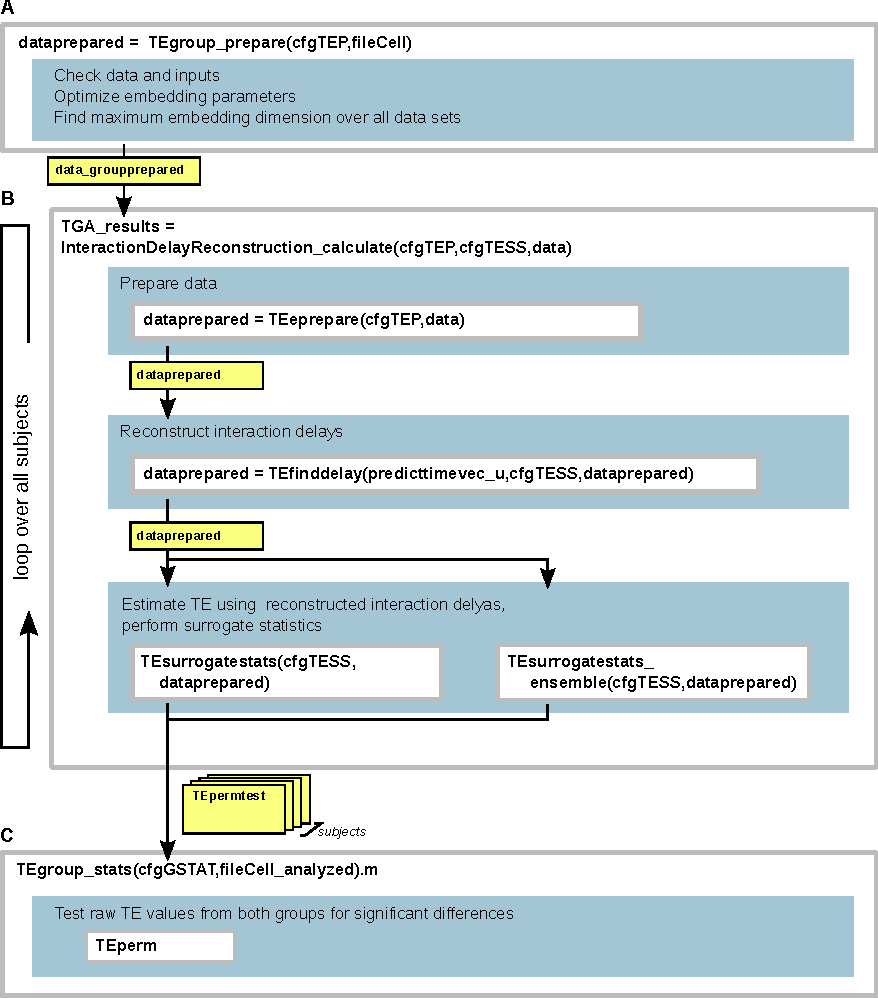
\includegraphics[scale=0.90]{figures/TRENTOOL3_groupanalysis.pdf}
	\caption[TRENTOOL work flow for group analysis]{TRENTOOL work flow for group analysis: 
	(A) All data sets have to be prepared for group analysis using the function \texttt{TEgroup\_prepare}, the function finds the maximum embedding dimension over all data sets/channel combinations and writes results to a field \texttt{groupprepare} in the data;
	(B) TE is estimated from group-prepared single subject data, the function  \texttt{InteractionDelayReconstruction\_calculate.m} recognizes data prepared for group analysis and uses group parameters from \texttt{data\_groupprepared.groupprepare} for TE analysis;
	(C) Raw TE values are compared between both groups by means of permutation testing, results are written to disk.
	}
	\label{fig:groupanalysis}
\end{figure} 


\subsubsection{\texttt{TEgroup\_prepare.m}}

\paragraph*{Description} The function prepares all data for group analysis (from both conditions/groups) by finding the group embedding dimension to be used for subsequent TE estimation. All data sets  are loaded by \verb&TEgroup_prepare.m& and passed to \verb&TEprepare.m& individually. From all individually optimal embedding parameters, the maximum embedding dimension is kept for subsequent TE analysis. Furthermore, the function checks whether all data sets use the same channel combination and assumed interaction delays $u$ to be scanned during TE estimation.

\paragraph*{Usage} \verb&data_groupprepared = TEgroup_prepare(cfgTEP,fileCell);&

\paragraph*{Input} \verb&fileCell& contains a cell array of file names (not paths, i.e. the function needs to be called from the folder containing the data sets), \verb&cfgTEP& contains a configuration structure with analysis parameters (table \ref{tab:cfgTEP}).

\paragraph*{Output} Results from \verb&TEgroup_prepare.m& are added to all data sets as an extra field \verb&.groupprepare& (table \ref{tab:groupprepare}). Data are then saved to a user specified location.

\subsubsection{Transfer entropy estimation} 

In its current version, TRENTOOL requires the use of the function \verb&InteractionDelayReconstruction_calculate.m& for TE estimation in group analysis. The function is called individually for each data set, prepared for group analysis. The work flow for TE analysis is the same as in single subject analysis (see section \ref{sec:interaction_delays}, \textit{Reconstruction of interaction delays}). Both the core TRENTOOL functions and the ensemble method for TE estimation (section \ref{sec:ensemble_method}) may be used. 

The function \verb&InteractionDelayReconstruction_calculate.m& recognizes data prepared for group analysis and replaces relevant fields in \verb&cfgTEP& with the group parameters found in \verb&data\_grouprepared.groupprepare& (embedding dimension and values for $u$ to be scanned). The function finds the optimal $u$ and estimates TE values using the optimal $u$ and group embedding parameters. TE estimates for individual data sets are returned to the user. 

\subsubsection{\texttt{TEgroup\_stats.m}}

\paragraph*{Description} The function compares the raw TE values estimated for all data sets and channel combinations by means of a permutation testing \cite{maris2007,lindner2011}. 

\paragraph*{Usage} \verb&TEgroup_stats(cfgGSTAT,fileCell_analyzed);& 

\paragraph*{Input} \verb&fileCell& contains a cell array of names of files that have been prepared for group analysis by running \texttt{TEgroup\_prepare.m} and have been analyzed individually, using the interaction delay reconstruction work flow (see \ref{sec:interaction_delays}). \verb&cfgGSTAT& contains a configuration structure with analysis parameters (table \ref{tab:cfgGSTAT}).

Subjects are assigned to groups using a design matrix specified in \texttt{cfgGSTAT.design} (table \ref{tab:ex_designmatrix}). The design matrix specifies group membership for statistical testing.

\begin{table}[H]
\small \centering
\caption[Example design matrix]{Example design matrix to be used in \texttt{cfgGSTAT.design} as a parameter for statistical testing in \texttt{TEgroup\_stats.m}. The first row holds the indices of data sets (in this case, two conditions are compared), the second row encodes the condition of the respective data set.} 
\begin{tabular}{|ll|cccccccccc|}  \hline
 dataset   & (\verb+uvar+) & 1 & 2 & 3 & 4 & 5 & 1 & 2 & 3 & 4 & 5 \\ \hline
 condition & (\verb+ivar+) & 1 & 1 & 1 & 1 & 1 & 2 & 2 & 2 & 2 & 2 \\ \hline
\end{tabular}\label{tab:ex_designmatrix}
\end{table}

\paragraph*{Output} The function \texttt{TEgroup\_stats.m} writes two files with suffixes \texttt{TE\_output.mat} and \texttt{TEpermtestgroup\_output.mat} to disc (location is specified in \texttt{cfgGSTAT.fileidout}). \texttt{TE\_output.mat} contains the raw TE values of both sets of data (\texttt{TEresult1} and \texttt{TEresult2}) as well as the mean over both sets (\texttt{TEresultmean}). \texttt{*TEpermtestgroup\_output.mat} contains the structure \texttt{TEpermtestgroup}, that holds the result of the statistical testing. Results are provided in the same fashion as for single subject analysis (see table \ref{tab:TEpermtest}), i.e. for each channel combination results of the permutation test are given in table form (\texttt{.TEpermvalues}). Additionally, the output structure contains a field \texttt{.TEgroupprepare}, that provides the results of \texttt{TEgroup\_prepare.m}.


\subsection{Graph correction for cascade effects and simple common drive} \label{sec:graphanalysis}

TRENTOOL allows for the partial correction of spurious information flow that may be introduced by bivariate analysis of a highly multivariate system. The description of the applied algorithm can be found in \cite{wollstadt2013}. The algorithm is provided in TRENTOOL as the function \verb&TEgraphanalysis.m& (Figure \ref{fig:graphanalysis}) and may be called on the output of any function that returns TE estimates: \verb&TEsurrogatestats.m&, \verb&TEsurrogatestats_ensemble.m&, and \verb&InteractionDelayReconstruction_calculate.m& (Figure \ref{fig:core_functions}). 


\subsubsection*{\texttt{TEgraphanalysis.m}}

\paragraph*{Description} The function corrects the network of significant information transfer for multivariate effects, namely cascade effects and simple common drive effects. The function tagss respective edges (significant information transfer between two time series) as potentially spurious and returns a modified output structure to the user.

\paragraph*{Usage} \verb&TEpermtest_GA = TEgraphanalysis(cfgGA,TEpermtest);&

\paragraph*{Input} \texttt{TEpermtest} can contain any structure with the field \verb&.TEpermvalues&, that is returned by one of the functions that handle TE estimation: \verb&TEsurrogatestats.m&, \verb&TEsurrogatestats_ensemble.m&, or \verb&InteractionDelayReconstruction_calculate.m&. \verb&cfgGA& contains a configuration structure with analysis parameters (table \ref{tab:cfgGA}).

\paragraph*{Output} The function returns the results structure that was used as input with a modified table in field \verb&.TEpermvalues& and a field \verb&.graphanalysis& with information on the information transfer network (table \ref{tab:graphanalysis_results}). 

\begin{figure}[H]	
	\centering 
 		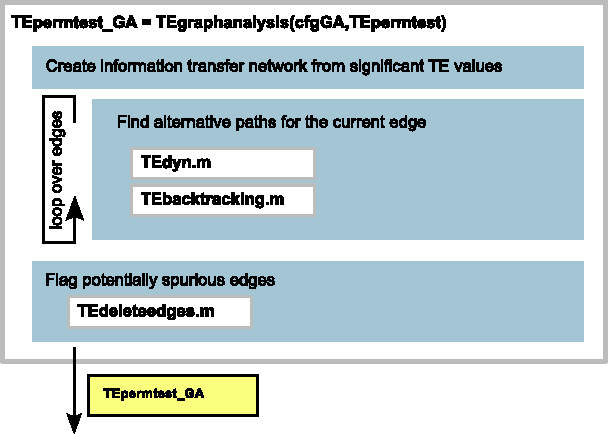
\includegraphics[width=0.75\textwidth]{figures/TRENTOOL3_graphanalysis.pdf}
	\caption[Graph based correction of spurious information transfer]{Post-hoc correction of spurious information transfer using a graph-based algorithm (correction for cascade effects and simple common drive).}
	\label{fig:graphanalysis}
\end{figure} 


\subsection{Plotting of TRENTOOL results}
%% TODO plotting routines

In the current version, TRENTOOL offers two options to visualize results from TE estimation. 

% \subsubsection{\texttt{InteractionDelayReconstruction\_plot.m}}
% 
% \paragraph*{Description} \texttt{InteractionDelayReconstruction\_plot.m} provides functionalities to plot TE values by assumed interaction delay $u$ for the reconstruction of interaction delays pipeline (see sec. \ref{sec:interaction_delays}, \textit{Reconstruction of interaction delays}). The function plots TE values for all assumed values $u$ returned by \texttt{InteractionDelayReconstruction\_calculate.m} and their respective significance levles (values $(1-p)$).
% 
% \paragraph*{Usage} \texttt{InteractionDelayReconstruction\_plot(cfgUPLOT);} 
% 
% \paragraph*{Input} \texttt{cfgUPLOT} contains a configuration structure with plotting parameters and path-/file-names (table \ref{tab:cfgUPLOT}).
% 
% \paragraph*{Output} The function plots normalized TE values ($TE/TE_{max}$) and significance levels ($1-p$). Significant information transfer is indicated by a black asterisk over the respective TE value. Volume conduction is indicated by a red asterisk. Note, that this function may produce a lot of figures, as individual plots are produced for all channel combinations.
%  % TODO find out, what this is supposed to do!

\subsubsection{\texttt{TEplot2D.m}}

\paragraph*{Description} \texttt{TEplot2D.m} plots the resulting network of information transfer for human neuronal data. The function plots results returned by functions \texttt{TEsurrogatestats.m}, \texttt{TEsurrogatestats\_ensemble.m}, \texttt{InteractionDelayReconstruction\_calculate.m} or \texttt{TEgroup\_stats.m}. Information transfer is plotted as arrows between sources or channels into a 2D head model.

\paragraph*{Usage} \texttt{InteractionDelayReconstruction\_plot(cfg2DPLOT,TEresult\_analyzed);} 

\paragraph*{Input} \texttt{cfg2DPLOT} contains a configuration structure with plotting parameters (table \ref{tab:cfg2DPLOT}), \texttt{TEresult\_analyzed} contains the structure \texttt{TEpermtest} returned by one of the above mentioned functions for TE analysis.

\paragraph*{Output} The function plots the network of information transfer using a user-provided layout of the sources. 

\subsubsection{\texttt{TRENTOOL2BrainNet.m}}

\paragraph*{Description} \texttt{TRENTOOL2BrainNet.m} exports results of TE estimation into a file format readable by BrainNet Viewer (\texttt{http://www.nitrc.org/projects/bnv/}, \cite{xia2013}). The function plots results returned by functions \texttt{TEsurrogatestats.m}, \texttt{TEsurrogatestats\_ensemble.m}, \texttt{InteractionDelayReconstruction\_calculate.m} or \texttt{TEgroup\_stats.m}. The function produces node and edge files, that can be read into BrainNet Viewer to produce 3D visualization of information transfer networks using MNI coordinates.

\paragraph*{Usage} \texttt{TRENTOOL2BrainNet(cfgBN,TEpermtest);} 

\paragraph*{Input} \texttt{cfgBN} contains a configuration structure with export parameters (table \ref{tab:cfgBN}), \texttt{TEpermtest} contains the structure \texttt{TEpermtest} returned by one of the above mentioned functions for TE analysis.

\paragraph*{Output} The function writes two files to disk: \texttt{*.node} and \texttt{*.edge}. \texttt{*.node} contains information regarding source positions in the 3D template in BrainNet Viewer. \texttt{*.edge} contains a connectivity matrix that defines the edges to be plotted by BrainNet Viewer (the label ordering corresponds to the ordering of sources in the \texttt{*.node}-file). See also the BrainNet Viewer manual (\url{http://www.nitrc.org/docman/view.php/504/1280/BrainNet Viewer Manual 1.42.pdf}).





\newpage
\section{Example scripts} \label{sec:example_scripts}

% \subsection{Example analysis main work flow}
% 
% \lstset{language=matlab,caption={Example script for the use of the main TRENTOOL work flow.},label=lst:mainTRENTOOLworkflow,breaklines=true,float=H,mathescape=true}
% \begin{lstlisting}
%% set paths

TRENTOOLpath = './TRENTOOL3';
addpath(TRENTOOLpath); 
addpath('./fieldtrip-20120703');
ft_defaults;

%% get data

% find relevant mat files and collect file names in a cell structure
files    = dir('subj_*.mat');

%% specify cfgTEP (parameters for TEprepare.m) 

cfgTEP                  = [];
cfgTEP.Path2TSTOOL      = './OpenTSTOOL';	% path to TSTOOL
cfgTEP.TEcalctype       = 'VW_ds'; 		% use the SPO estimator

load(files(1).name);
cfgTEP.channel       = data.label; 	% analyze all combinations of channels in the field label
cfgTEP.predicttime_u = 12;  		% known interaction delay
cfgTEP.toi  	     = [min(data.time{1,1}),max(data.time{1,1})]; % analysis window/time of interest

cfgTEP.maxlag      = 10000;   % range for ACT computation
cfgTEP.actthrvalue = 120;     % treshold for ACT 
cfgTEP.minnrtrials = 12;      % minimum acceptable number of trials

% optimizing embedding
cfgTEP.optimizemethod ='ragwitz';   % criterion used
cfgTEP.ragdim         = 2:8;        % criterion dimension
cfgTEP.ragtaurange    = [0.5 1];    % range for tau 
cfgTEP.ragtausteps    = 15;         % steps for ragwitz tau steps
cfgTEP.repPred        = 1000;       % points to be predicted

% kernel-based TE estimation
cfgTEP.flagNei = 'Mass' ;           % neigbour analyse type
cfgTEP.sizeNei = 4;                 % neigbours to analyse

%% prepare data for TE estimation

for i=1:length(files)

  load(files(i).name);
  dataprepared = TEprepare(cfgTEP,data);
  
  save([files(i).name(1:end-4) '_prepared.mat'],'dataprepared');
end


%% specify cfgTESS (parameters for TEsurrogatestats.m) 

cfgTESS = [];

cfgTESS.optdimusage = 'indivdim';   % dimension to use

% options for statistical testing
cfgTESS.tail           = 1;
cfgTESS.numpermutation = 5e4;
cfgTESS.shifttesttype  = 'TEshift>TE';
cfgTESS.surrogatetype  = 'trialshuffling';

% addiotional condition for TE calculation
%cfgTESS.extracond = 'Faes_Method';	% extracond and shift testing are mutually exclusive

files = dir('*_prepared.mat');

for i=1:length(files)
  
  % load prepared data
  load(files(i).name)
  
  % filename under which auxiliary data is saved by TEsurrogatestats.m
  cfgTESS.fileidout = ['results/ ' files(i).name(1:end-13)];
  
  TEresult = TEsurrogatestats(cfgTESS,dataprepared);
  
  save([cfgTESS.fileidout '_analyzed.mat'],'TEresult');
end  


%% Graph analysis (optional) 

files = dir('*_analyzed.mat');

% specify parameters for graph analysis
cfgGA = [];
cfgGA.threshold = 3; % threshold for alternative path search in msec

for i=1:length(files)
  
  % load prepared data
  load(files(i).name)
  
  TEresult_GA = TEgraphanalysis(cfgGA,TEresult);
  
  save([cfgTESS.fileidout '_analyzed_GA.mat'],'TEresult_GA');
end  
\end{lstlisting}


\subsection{Example analysis: Interaction delay reconstruction}

The following example script uses the functions \texttt{InteractionDelayReconstruction\_*} for the reconstruction of interaction delays together with the core TRENTOOL functions for TE estimation. The example script \texttt{example\_script\_CPUmethod.m} and data \texttt{exampledata/Lorenz\_1->2\_45ms.mat} can be found in the current TRENTOOL version.

\lstset{language=matlab,caption={Example script for interaction delay reconstruction in TRENTOOL, using the core TRENTOOL functions for TE estimation.}, label=lst:delayreconstruction_CPU,breaklines=true,float=H,mathescape=true}
\begin{lstlisting}
%% set paths

addpath('../TRENTOOL3')
addpath('../fieldtrip-20150928');
ft_defaults;

%% define data paths

OutputDataPath = '../results/';
InputDataPath  = 'exampledata/Lorenz_1->2_45ms.mat';

load(InputDataPath);


%% define cfg for TEprepare.m

cfgTEP = [];

% data
cfgTEP.toi                 = [min(data.time{1,1}),max(data.time{1,1})]; % time of interest
cfgTEP.sgncmb              = {'A1' 'A2'};  % channels to be analyzed

% scanning of interaction delays u
cfgTEP.predicttimemin_u    = 40;      % minimum u to be scanned
cfgTEP.predicttimemax_u    = 50;	  % maximum u to be scanned
cfgTEP.predicttimestepsize = 1; 	  % time steps between u's to be scanned

% estimator
cfgTEP.TEcalctype  = 'VW_ds'; % use the new TE estimator (Wibral, 2013)

% ACT estimation and constraints on allowed ACT(autocorelation time)
cfgTEP.actthrvalue = 100;   % threshold for ACT
cfgTEP.maxlag      = 1000;
cfgTEP.minnrtrials = 15;   % minimum acceptable number of trials

% optimizing embedding
cfgTEP.optimizemethod ='ragwitz';  % criterion used
cfgTEP.ragdim         = 2:9;       % criterion dimension
cfgTEP.ragtaurange    = [0.2 0.4]; % range for tau
cfgTEP.ragtausteps    = 5;        % steps for ragwitz tau steps
cfgTEP.repPred        = 100;      % size(data.trial{1,1},2)*(3/4);

% kernel-based TE estimation
cfgTEP.flagNei = 'Mass' ;           % neigbour analyse type
cfgTEP.sizeNei = 4;                 % neigbours to analyse


%% define cfg for TEsurrogatestats_ensemble.m

cfgTESS = [];

% use individual dimensions for embedding
cfgTESS.optdimusage = 'indivdim';

% statistical and shift testing
cfgTESS.tail           = 1;
cfgTESS.numpermutation = 5e4;
cfgTESS.shifttesttype  ='TEshift>TE';
cfgTESS.surrogatetype  = 'trialshuffling';

% results file name
cfgTESS.fileidout  = strcat(OutputDataPath,'Lorenzdata_1->2_');

%% calculation - scan over specified values for u

TGA_results = InteractionDelayReconstruction_calculate(cfgTEP,cfgTESS,data);

save([OutputDataPath 'Lorenz_1->2_TGA_results.mat'],'TGA_results');

%% optional: perform a post hoc correction for cascade effects and simple common drive effects

cfgGA = [];

cfgGA.threshold = 3;
cfgGA.cmc = 1;

TGA_results_GA = TEgraphanalysis(cfgGA,TGA_results_analyzed);

save([OutputDataPath 'Lorenz_1->2_TGA_results_analyzed_GA.mat'],'TGA_results_GA');



%% plotting

load('exampledata/Lorenz_layout.mat');

cfgPLOT = [];

cfgPLOT.layout        = lay_Lorenz; 		% see fieldtrip's ft_prepare_layout.m
cfgPLOT.electrodes    = 'highlights';
cfgPLOT.statstype     = 1;   		% 1: corrected; 2:uncorrected; 3: 1-pval; 4:rawdistance
cfgPLOT.alpha         = 0.05;
cfgPLOT.arrowpos      = 1;
cfgPLOT.showlabels    = 'yes';
cfgPLOT.electrodes    = 'on';
cfgPLOT.hlmarker      = 'o';
cfgPLOT.hlcolor       = [0 0 0];
cfgPLOT.hlmarkersize  = 4;
cfgPLOT.arrowcolorpos = [1 0 0];

figure; 
TEplot2D(cfgPLOT,TGA_results_analyzed_GA)
\end{lstlisting}




\subsection{Example analysis: Interaction delay reconstruction with ensemble method for TE estimation}

The following example script uses the ensemble method for TE estimation together with functions \texttt{InteractionDelayReconstruction\_*} for the reconstruction of interaction delays. Note, that in comparison to the first example script, the ensemble method allows for the analysis of shorter time windows of interest (in the example, '\verb&toi&' is set to 120 msec). These short analysis windows can typically not be realized without the use of the ensemble method as the number of data points is not sufficient.

To account for the shorter analysis windows and the reduction in data points per repetition, parameters for the embedding optimization have to be adjusted (e.g. \verb&cfgTEP.maxlag& or \verb&cfgTEP.repPred&).

The example script \texttt{example\_script\_ensemblemethod.m} and data \texttt{exampledata/Lorenz\_1->2\_45ms.mat} can be found in the current TRENTOOL version.

\lstset{language=matlab,caption={Example script for interaction delay reconstruction in TRENTOOL.},label=lst:delayreconstruction_GPU,breaklines=true,float=H,mathescape=true}
\begin{lstlisting}
%% set paths

addpath('../TRENTOOL3')             % note: this script assumes, you have already compiled the GPU mex-files using 'install.m'
addpath('../fieldtrip-20150928');
ft_defaults;

%% define data paths

OutputDataPath = '../results/';
InputDataPath  = 'exampledata/Lorenz_1->2_45ms.mat';

load(InputDataPath);

%% define cfg for TEprepare.m

cfgTEP = [];

% data
cfgTEP.toi                 = [min(data.time{1,1}),max(data.time{1,1})]; % time of interest
cfgTEP.sgncmb              = {'A1' 'A2'};  % channels to be analyzed

% scanning of interaction delays u
cfgTEP.predicttimemin_u    = 40;		  % minimum u to be scanned
cfgTEP.predicttimemax_u    = 50;	  % maximum u to be scanned
cfgTEP.predicttimestepsize = 1; 	  % time steps between u's to be scanned

% estimator
cfgTEP.TEcalctype  = 'VW_ds'; % use the new TE estimator (Wibral, 2013)

% use ensemble method
cfgTEP.ensemblemethod = 'yes';

% ACT estimation and constraints on allowed ACT(autocorelation time)
cfgTEP.actthrvalue = 40;   % threshold for ACT
cfgTEP.maxlag      = 100;
cfgTEP.minnrtrials = 15;   % minimum acceptable number of trials

% optimizing embedding
cfgTEP.optimizemethod ='ragwitz';  % criterion used
cfgTEP.ragdim         = 2:8;       % criterion dimension
cfgTEP.ragtaurange    = [0.2 0.4]; % range for tau
cfgTEP.ragtausteps    = 15;        % steps for ragwitz tau steps
cfgTEP.repPred        = 100;       % points used for optimization the embedding dimensions

% kernel-based TE estimation
cfgTEP.flagNei = 'Mass' ;           % neigbour analyse type
cfgTEP.sizeNei = 4;                 % neigbours to analyse


%% define cfg for TEsurrogatestats_ensemble.m

cfgTESS = [];

% use individual dimensions for embedding
cfgTESS.optdimusage = 'indivdim';

% surrogate testing
cfgTESS.tail           = 1;
cfgTESS.surrogatetype  = 'trialperm';
cfgTESS.numpermutation = 100;

% GPU specifications
cfgTESS.GPUmemsize     = 4200;
cfgTESS.numthreads     = 512;
cfgTESS.maxgriddim     = 65535;

% volume conduction
cfgTESS.extracond      = 'Faes_Method';
cfgTESS.shifttest      = 'no';

% calculation of mutual information (MI)
cfgTESS.MIcalc = 1;

% results file name
cfgTESS.fileidout  = strcat(OutputDataPath,'Lorenzdata_1->2_ensemble_');


%% calculation - scan over specified values for u

TGA_results = InteractionDelayReconstruction_calculate(cfgTEP,cfgTESS,data);

save([OutputDataPath 'TGA_results.mat'],'TGA_results');


%% optional: perform a post hoc correction for cascade effects and simple common drive effects

cfgGA = [];

cfgGA.threshold = 3;
cfgGA.cmc = 1;

TGA_results_GA = TEgraphanalysis(cfgGA,TGA_results);

save([OutputDataPath 'Lorenz_1->2_TGA_results_analyzed_GA.mat'],'TGA_results_GA');



%% plotting

load('exampledata/Lorenz_layout.mat');

cfgPLOT = [];

cfgPLOT.layout        = lay_Lorenz; 		% see fieldtrip's ft_prepare_layout.m
cfgPLOT.electrodes    = 'highlights';
cfgPLOT.statstype     = 1;   		% 1: corrected; 2:uncorrected; 3: 1-pval; 4:rawdistance
cfgPLOT.alpha         = 0.05;
cfgPLOT.arrowpos      = 1;
cfgPLOT.showlabels    = 'yes';
cfgPLOT.electrodes    = 'on';
cfgPLOT.hlmarker      = 'o';
cfgPLOT.hlcolor       = [0 0 0];
cfgPLOT.hlmarkersize  = 4;
cfgPLOT.arrowcolorpos = [1 0 0];

figure; 
TEplot2D(cfgPLOT,TGA_results_analyzed_GA)
\end{lstlisting}


\subsection{Example group analysis}

\lstset{language=matlab,caption={Example script for group analysis in TRENTOOL.},label=lst:groupanalysis,breaklines=true,float=H,mathescape=true}
\begin{lstlisting}
%% set paths

TRENTOOLpath = './TRENTOOL3';
addpath(TRENTOOLpath); 
addpath('./fieldtrip-20150928');
ft_defaults;

%% get data

% find relevant mat files and collect file names in a cell structure
files    = dir('subj_*.mat');
fileCell = {files(:).name};

%% create cfg (as you would for single subject analysis)

cfgTEGP                  = [];
cfgTEGP.TEcalctype       = 'VW_ds'; 

% get channel label from file, analyze all possible combinations
load(files(1).name);
cfgTEP.channel             = data.label;

% specify u to be scanned
cfgTEGP.predicttimemin_u    = 5;
cfgTEGP.predicttimemax_u    = 17;
cfgTEGP.predicttimestepsize = 2;

% use the whole trial for analysis
cfgTEP.toi = [min(data.time{1,1}),max(data.time{1,1})]; % time of interest

% ACT estimation and constraints on allowed ACT(autocorelation time)
cfgTEGP.maxlag      = 3*cfgTEGP.predicttimemax_u;   % range for ACT computation
cfgTEGP.actthrvalue = 40;                           % treshold for ACT 
cfgTEGP.minnrtrials = 12;                           % minimum acceptable number of trials

% optimizing embedding
cfgTEGP.optimizemethod ='ragwitz';   % criterion used
cfgTEGP.ragdim         = 4:8;        % criterion dimension
cfgTEGP.ragtaurange    = [0.2 0.4];  % range for tau [0.5 1]
cfgTEGP.ragtausteps    = 15;         % steps for ragwitz tau steps
cfgTEGP.repPred        = 100;        % points used for optimization the embedding dimensions

% kernel-based TE estimation
cfgTEGP.flagNei = 'Mass' ;           % neigbour analyse type
cfgTEGP.sizeNei = 4;                 % neigbours to analyse

cfgTEGP.ensemblemethod  = 'no';
cfgTEGP.outputpath  = '/results/';

%% run TEgroup_prepare

TEgroup_prepare(cfgTEGP,fileCell);

%% run analysis on group prepared data

cfgTESS		      = [];
cfgTESS.shifttest     = 'yes';
cfgTESS.optdimusage   = 'indivdim';   % dimension to use
cfgTESS.surrogatetype = 'trialshuffling';

% go to output path of previous analysis step (this is where TEgroup_prepare saved the prepared data)
cd(cfgTEGP.outputpath)

% load and analyze prepared data individually
for i=1:length(fileCell)
        
    load(fileCell(i).name)
    cfgTESS.fileidout = strcat(cfgTEGP.outputpath,fileCell(i).name(1:5));
    
    TEresult = InteractionDelayReconstruction_calculate(cfgTEGP,cfgTESS,data);
    
    save([cfgTEGP.outputpath fileCell(i).name(1:end-4) '_calc.mat'],'TEresult');
    clear TEresult data;
    
end

%% perform graph analysis (optional)

files = dir('*_calc.mat');


% settings for graph analysis
cfgGA = [];
cfgGA.threshold = 1;
cfgGA.cmc       = 1;

for i=1:length(files)
    
    load(files(i).name);
    
    % correct for spurious information transfer
    TEresult_GA = TEgraphanalysis(cfgGA,TEresult);
    
    save([cfgTEGP.outputpath files(i).name(1:end-9) '_result.mat'],'TEresult_GA');
    
end


%% run group statistics

% collect individually analyzed data in a file cell
cd(cfgTEGP.outputpath);
fileCell_TEpermtest = dir('*_result.mat');
fileCell_TEpermtest = {fileCell_TEpermtest(:).name};

% define analysis parameters
cfgGSTAT = [];
cfgGSTAT.design    = [1 2 3 4 5 6 7 8; 1 1 1 1 2 2 2 2];
cfgGSTAT.uvar      = 1;
cfgGSTAT.ivar      = 2;
cfgGSTAT.permstatstype = 'indepsamplesT';
cfgGSTAT.fileidout = 'test_groupstats';

% run group statistics
TEgroup_stats(cfgGSTAT,fileCell_TEpermtest);
\end{lstlisting}


\newpage
\section{Appendix} \label{sec:appendix}

The following tables provide detailed information on input and output of the most common TRENTOOL functions. Input parameters are mandatory if no default values are provided. Curly brackets indicate MATLAB cell arrays, square brackets indicate numeric arrays. Note, that MATLAB uses row-major order for multidimensional arrays.


\onehalfspacing

% TEprepare
\begin{table}[H]
\small
\caption[Parameters \texttt{cfgTEP}]{Prameters for the configuration structure \texttt{cfgTEP.} of the functions \texttt{TEprepare.m}, \texttt{TEgroup\_prepare.m} and \texttt{InteractionDelayReconstruction\_calculate} (TRENTOOL Version 3.3)} 
\makebox[\textwidth]{
\begin{tabularx}{1.1\textwidth}{lp{1.2cm}L{1.3cm}p{1.1cm}X}\toprule 
\label{tab:cfgTEP}
\textbf{field name}& \textbf{default value} & \textbf{data type} & \textbf{units} & \textbf{description} \\ \midrule
\rowcolor{Gray}
\verb+sgncmb+ & & string & & cell array of channel pairs to be analyzed\\
\verb+channel+ & & string & & cell array of channel names, from which TRENTOOL will construct all possible pairs for later analysis\\
%\verb+Path2TSTOOL+ & & string & & path to the folder including the required TSTOOL package\\
\rowcolor{Gray}
\verb+toi+ & & double & seconds & 1x2-vector with first and last time point of the time range of interest \\
\verb+TEcalctype+ & \verb+'VW_ds'+ & string & & \texttt{'VW\_ds'}: Estimator guaranteeing optimal self prediction (eq. \ref{eq:TE_u}, see \cite{wibral2013}). \verb+'V'+ and \verb+'VW'+ estimators are no longer supported\\
\rowcolor{Gray}
\verb+predictiontime_u+ & & integer & milli-seconds & assumed information transfer delay $u$ between source and target time series (Fig. \ref{fig:TE_concept}) \\
\verb+ensemblemethod+ & \verb+'no'+ & string & & Use of the ensemble-method for (time-resolved) TE estimation, see sec. \ref{sec:ensemble_method} \cite{wollstadt2013} (\verb+'yes'+ or \verb+'no'+). \\
\rowcolor{Gray}
\verb+kth_neighbors+ & \verb+4+ & integer & & number of neighbors for fixed mass search (controls balance of bias/statistical errors) \\
\verb+TheilerT+ & \verb+'ACT'+ & integer or string 'ACT' & & number of temporal neighbors excluded to avoid serial correlations (Theiler correction)\\
\rowcolor{Gray}
\verb+maxlag+ & \verb+1000+ & integer & samples & the range of lags for computing the ACT: from -MAXLAG to MAXLAG \\ 
\verb+optimizemethod+ & & string & & define method for parameter optimization: 'ragwitz' \\%or 'cao'\\
\rowcolor{Gray}
\verb+trialselect+ & \verb+'ACT'+ & string & & selecting trials: 'no' uses all available trials, 'range' uses trials from a separately defined range (fields \texttt{.trial\_from} and \texttt{trial\_to}), 'ACT' uses trials with an ACT lower than a given threshold (field \texttt{.actthresholdvalue})\\
\verb+actthrvalue+ & & integer & & max threshold for the ACT for trial selection\\
\rowcolor{Gray}
\verb+trial_from+ & & integer & & first trial in case of range selection of trials\\
\verb+trial_to+ & & integer & & last trial in case of range selection of trials\\
\rowcolor{Gray}
\verb+minnrtrials+ & & integer & & sets a minimum number of trials, that have to survive trial selection (if \verb+cfgTEP.trialselect = 'ACT'+ is set); if less trials survive trial selection, TE estimation is abortet\\ 
\verb+verbosity+ & \verb+'info_minor'+ & string & & defines the verbosity of console output of TRENTOOL (see section \ref{sec:verbosity})\\
\multicolumn{5}{l}{}\\
\multicolumn{5}{l}{\textbf{Parameters needed for the use of Ragwitz' criterion for parameter optimization}}\\ \midrule
\verb+ragdim+ & \verb+1 to 10+ & integer & & for Ragwitz: range of embedding dimensions to scan vector from 1 to n\\
\rowcolor{Gray}
\verb+ragtaurange+ & & double & units of act & for Ragwitz: 1x2-vector of min and max embedding delays \\
\verb+ragtausteps+ & \verb+10+  & integer & &  for Ragwitz: number of equidistant steps in ragtaurange with a minimum of 5\\
\rowcolor{Gray}
\verb+flagNei+ & & string & & for Ragwitz: 'Range' or 'Mass' type of neighbor search\\
\verb+sizeNei+ & & integer & & for Ragwitz: Radius or mass for the neighbor search according to \verb+flagNei+\\
\rowcolor{Gray}
\verb+repPred+ & & integer & & for Ragwitz: repPred represents the number of sample points for which the prediction is performed (it has to be smaller than $length(timeSeries)-(embedding dimension-1)*tau*ACT-u$ )\\ \bottomrule
% \multicolumn{5}{l}{}\\
% \multicolumn{5}{l}{\textbf{Parameters needed for the use of Cao criterion for parameter optimization$^{a}$}}\\ \midrule
% \verb+caodim+ & \verb+1 to 10+ & integer & & for Cao: indicates the range of dimensions that is scanned using the Cao criterion to find the optimal dimension \\
% \rowcolor{Gray}
% \verb+caokth_neighbors+ & \verb+4+ & integer & & for Cao: number of neighbors for fixed mass search for cao (controls balance of bias/statistical errors) \\
% \verb+tau+ & \verb+1.5+ & double & units of act & for Cao: embedding delay \\ 
% \multicolumn{5}{p{\textwidth}}{$^a$ The cao criterion is not recommended for parameter optimization. The code for cao-optimization is no longer maintained and guaranteed to work vor TRENTOOL versions 3.0 and higher.}
\end{tabularx}}
\end{table} % parameters for cfgTEP

\begin{table}[H]
%\centering
\caption[Results \texttt{.TEprepare}]{Results provided in the field \texttt{.TEprepare}, added to the data by \texttt{TEprepare.m} (TRENTOOL Version 2.0)} % TODO update this to version 3
\makebox[\textwidth]{
\begin{tabularx}{1.1\textwidth}{p{3cm}L{3cm}p{1.5cm}p{1.1cm}X} \toprule
\textbf{field name} & \textbf{dimension} & \textbf{data type} & \textbf{units} & \textbf{description} \\ \midrule
 \texttt{channelcombi} & [no. channel combinations x 2] & integers & & cell array with channel indices specifying the channel combinations to be analyzed\\
 \rowcolor{Gray}
 \texttt{channelcombilabel} & \{no. channel combinations x 2 \} & strings & & cell array with channel labels specifying the channel combinations to be analyzed\\
 \texttt{ACT} & [no. channel combinations x 2 x no. trials] & integers & samples & array with the values of the auto correlation decay times of the channelcombinations\\
 \rowcolor{Gray}
 \texttt{trials} & \{no. channel combinations x 2\} [1 x no. trials] & integers & & cell array of integer arrays containing trials used for individual channel combinations for analysis\\
 \texttt{ntrials} & [no. channel combinations x 2] & integers & & integer array containing the number of trials used for individual channel combinations for analysis\\
 \rowcolor{Gray}
 \texttt{optdimmattrial} & [channelcombi x trial] & integer & & array with optimal embedding dimension for each trial\\
 \texttt{optdimmat} & [channelcombi x 1] & integer & & array with optimal embedding dimension for each channel combination (over trials)\\
 \rowcolor{Gray}
 \texttt{optdim} & scalar & integer & & max of the \texttt{optdimmat} which should be used as embedding dimension in the further steps\\
 \texttt{timeindices} & [1 x 2] & integer & samples & timeindices in samples (from \texttt{cfg.toi})\\
 \rowcolor{Gray}
 \texttt{u\_in\_samples} & scalar & integer & samples & interaction delay in sample points (from \texttt{cfg.predictionstime\_u})\\
 \texttt{cfg} & & structure & & configuration structure \texttt{cfgTEP} (table \ref{tab:cfgTEP}) provided by the user\\
 \rowcolor{Gray}
\texttt{maxact} & scalar & integer & & maximum autocorrelation decay time of the targetchannels\\ 
%\multicolumn{5}{l}{}\\
%\multicolumn{5}{l}{\textbf{Parameters returned if ragwitz criterion was chosen for parameter optimization}}\\ \midrule
\texttt{opttaumat} & [1 x channelcombi] & integer & & optimal embedding delays tau for each channel combination over trials\\
\rowcolor{Gray}
\texttt{opttau}  & scalar & integer & & max of the opttaumat which should be used as embedding delay in the further steps\\ \bottomrule
% \multicolumn{5}{l}{}\\
% \multicolumn{5}{l}{\textbf{Parameters returned if cao criterion was chosen for parameter optimization$^a$}}\\\midrule
% \texttt{nrreferencepoints} & [no. channel combination x no. trial] & integer & & number of reference points for the cao calculation\\
% \rowcolor{Gray}
% \texttt{cao} & & structure & & Contains two arrays [no trials x no. channels x caodim] with the values E1 and E2 of the cao function\\ \bottomrule
% \multicolumn{5}{p{\textwidth}}{$^a$ The cao criterion is not recommended for parameter optimization. The code for cao-optimization is no longer maintained and guaranteed to work vor TRENTOOL versions 3.0 and higher.}
\end{tabularx}} \label{tab:TEprepare}
\end{table}
 % results returned by TEprepare 

% TEsurrogatestats
\begin{table}[H]
\small
\caption[Parameters \texttt{cfgTESS}]{Parameters for the configuration structure \texttt{cfgTESS} of the functions \texttt{TEsurrogatestats.m}, \texttt{TEsurrogatestats\_ensemble.m} and \texttt{InteractionDelayReconstruction\_calculate.m} (TRENTOOL Version 3.3)} 
\makebox[\textwidth]{
\begin{tabularx}{1.1\textwidth}{p{2cm}p{2cm}p{1.1cm}X} \toprule
\textbf{field name} & \textbf{default value} & \textbf{data type} & \textbf{description} \\ \midrule
\verb+optdimusage+ & & string & 'maxdim' to use maximum of optimal embedding dimensions over all channels for all channels, or 'indivdim' to use the individual optimal dimension for each channel. In case of using ragwitz criterion also the optimal embedding delay tau per channelcombi is used. \\
\rowcolor{Gray}
\verb+dim+ & output TEprepare & integer & Value(s) for embedding dimension. This is automatically taken from the field \verb+TEprepare+ in the data (recommended!). Otherwise: scalar value (if \verb+cfgTESS.optdimusage = 'maxdim'+) or vector of size [channelcombi x 1] (if \verb+cfgTESS.optdimusage = 'indivdim'+).\\
\verb+tau+ & output TEprepare & integer & Embedding delay in units of act (x*act). This is automatically taken from the field \verb+TEprepare+ in the data (recommended!). Otherwise: scalar value (if \verb+cfgTEP.optdimusage = 'maxdim'+) or vector of size [channelcombi x 1] (if \verb+cfgTEP.optdimusage = 'indivdim'+). Otherwise: \\ %TODO tau???
\rowcolor{Gray}
\verb+alpha+ & 0.05 & double & Significance level for statisatical permutation test \\
\verb+surrogatetype+ & & string & Strategy for surrogate data creation: 'trialshuffling', 'trialreverse', 'blockresampling', 'blockreverse1','blockreverse2', or 'blockreverse3' (see section \ref{sec:TEsurrogatestats}).\\
\rowcolor{Gray}
\verb+extracond+ & & string & Perform conditioning in tansfer entropy formula on additional variables. Values: \verb+'Faes_Method'+ (\cite{faes2013}, see section \ref{sec:TEsurrogatestats}) \\
\verb+MIcalc+ & 1 & integer & Determines whether mutual information is calculated additionally to TE (1) or not (0).\\
\rowcolor{Gray}
\verb+shifttest+ & 'yes' & string & Perform shift test to identify instantaneous mixing between the signal pairs. Values: 'yes' or 'no'. Note: If \verb+cfgTESS.extracond = 'Faes_Method'+ is requested, \texttt{cfgTESS.shifttest} has to be set to 'no' as both methods are mutually exclusive (see section \ref{sec:TEsurrogatestats}).\\
\verb+shifttesttype+ & 'TE>TEshift' & string & The shift test can be calculated for the direction TE value of original data > TE values of shifted data (value = 'TE>TEshift') or for the other direction (value = 'TEshift>TE'). In this case the alpha is set to 0.1.\\
\rowcolor{Gray}
\verb+shifttype+ & 'predicttime'& string & Shifting the data 'onesample' or the length of the 
'predicttime'. \\
\verb+numpermutation+ & 190100/500$^a$ & integer & Nr of permutations in permutation test.\\
\rowcolor{Gray}
\verb+permstatstype+  & 'indepsamplesT' & string & Type of the test statistic used: 'mean' to use the distribution of the mean differences, 'normmean' to use the distribution of the normalized mean differences and 'depsamplesT' or 'indepsamplesT' for distribution of the t-values.\\
\verb+tail+ & 1 & integer & 1 tail or 2 tailed test of significance (for the permutation tests).\\
\rowcolor{Gray}
\verb+correctm+ & 'FDR' & string & Correction method used for correction of the multiple comparison problem over all analyzed channel combinations - False discovery rate 'FDR' or Bonferroni correction 'BONF'.\\
\verb+fileidout+ & & string & String for the first part of the output filename.\\
\multicolumn{4}{l}{}\\
\multicolumn{4}{l}{\textbf{Additional hardware parameters needed when using the ensemble method for TE estimation}}\\ \midrule
\rowcolor{Gray}
\verb+GPUmemsize+ & & integer & The memory of the GPU in MB (e.g. \verb+cfg.GPUmemsize = 4200;+). \\
\verb+numthreads+ & & integer & Max. number of threads that can be run in one block on the GPU. \\
\rowcolor{Gray}
\verb+maxgriddim+ & & integer & Max. grid dimension of the GPU. \\
\bottomrule
\multicolumn{4}{p{\textwidth}}{$^a$ The first value is the default for trial-wise TE estimation on the CPU, the second value is the default for ensemble TE estimation using a GPU.}
\end{tabularx}} \label{tab:cfgTESS}
\end{table} % parameters for cfgTESS
\begin{table}[H]
\centering
\caption[Results \texttt{TEpermtest}]{Results provided in the structure \texttt{TEpermtest} saved to disk/returned by '\texttt{TEsurrogatestats.m}' and '\texttt{TEsurrogatestats\_ensemble.m}', (TRENTOOL Version 3.3)}
\begin{tabularx}{\textwidth}{lL{2.5cm}L{2.5cm}X}\toprule
\textbf{field name} & \textbf{dimension} & \textbf{data type} & \textbf{description} \\ \midrule
\texttt{dimord} & & string & dimensions of TEpermvalues \\
\rowcolor{Gray}
\texttt{cfg} & & structure & configuration file used to TE estimation (\texttt{cfgTESS}, see table \ref{tab:cfgTESS}) \\
\texttt{sgncmb} & & cell array of strings & labels of channel combinations (source -> target) \\
\rowcolor{Gray}
\texttt{numpermutation} & scalar & integer & number of permutations used for statistical testing \\
\texttt{ACT} & & structure & structure including \texttt{.act} with the ACT matrix ([channelcombi x 2 x trial]) \\
\rowcolor{Gray}
\texttt{nr2cmc} & scalar & integer & number of of multiple comparisons that was corrected for \\
\texttt{TEprepare} & & structure & results of the function TEprepare from the input data \\ 
\rowcolor{Gray}
\texttt{TEpermvalues} & [no. channel combinations x 5(6$^a$)] & doubles & matrix with results of permutation testing for individual channel combinations. For each channel combination (i.e. each row), the matrix holds the following information: \\ 
&&&\\
& \textbf{Column} & \textbf{Description} & \textbf{Values} \\ \midrule
 &1 & p-value & $0$ to $1$ \\
 \rowcolor{Gray}
 &2 & stat. significance & $1$ significant at the provided alpha level, $0$ not significant \\ 
 &3 & stat. significance after CMC$^b$& $1$ significant at the provided alpha level after CMC, $0$ not significant after CMC\\ 
 \rowcolor{Gray}
 &4 & mean difference & raw difference between empirical and surrogate data \\ 
 &5 & volume conduction & indicates the presence ($1$) or absense ($0$) of volume conduction (is set to $NaN$ for ensemble method) \\
 \rowcolor{Gray}
 &6$^a$ & optimal $u$ & $u$ in msec, available only after  was ran on data\\ \bottomrule
\multicolumn{4}{p{\textwidth}}{$^a$ a sixth column containing the optimal $u$ is added only if interaction delays are reconstructed for the data (using \texttt{InteractionDelayReconstruction\_analyze.m}, see section \ref{sec:interaction_delays})}\\
\multicolumn{4}{p{\textwidth}}{$^b$ correction for multiple comparisons}\\
\end{tabularx} \label{tab:TEpermtest}
\end{table}
 % results returned in TEpermvalues
\begin{table}[H]
\centering
\caption[Results \texttt{TEresult}]{Results provided in the structure \texttt{TEresult} saved to disk by '\texttt{TEsurrogatestats.m}' and '\texttt{TEsurrogatestats\_ensemble.m}' (TRENTOOL Version 3.3)}
\begin{tabularx}{\textwidth}{lL{2.5cm}L{2cm}X}\toprule
\textbf{field name} & \textbf{dimension} & \textbf{data type} & \textbf{description} \\ \midrule
\texttt{TEmat} & [no. channel combinations x u x trial] & double & matrix of raw TE values \\ 
	       & [no. channel combinations] & double & vector of raw TE values if the ensemble method is used for TE estimation\\ 
\rowcolor{Gray}
\texttt{MImat} & [no. channel combinations x u x trial] & double & matrix of rax mutual information values\\
\rowcolor{Gray}
	       & [no. channel combinations] & double & vector of raw MI values if the ensemble method is used for TE estimation\\ 
\texttt{dimord} & & string &  dimension of TEmat and MImat\\
\rowcolor{Gray}
\texttt{cfg} &  & structure & configuration structure used for TE estimation (\texttt{cfgTESS}, see table \ref{tab:cfgTESS}) \\
\texttt{trials} & & & trial numbers selected from raw data set \\
\rowcolor{Gray}
\texttt{act} & [no. channel combinations x 2 x no. trials] & integer & ACT matrix\\
\texttt{sgncmb} & & structure & results of the function TEprepare from the input data \\ 
 \bottomrule
\end{tabularx} \label{tab:TEresult}
\end{table}
 % results saved in TEresult % TODO check if this u dimension is still in there -> same for MI, check missing dimensions

% InteractionDelayReconstruction_analyze
%\begin{table}[H]
\small
\caption[Parameters \texttt{cfgTEA}]{Parameters for the configuration structure \texttt{cfgTEA} of the function \texttt{InteractionDelayReconstruction\_analyze.m} (all parameters are given as strings) (TRENTOOL Version 3.0)} 
\begin{tabularx}{\textwidth}{lX} \toprule
\textbf{field name} & \textbf{description} \\ \midrule
\verb+select_opt_u+ & selects the way the optimal u is determined options are: \\
                 &        \verb+'min_p'+ - optimal predictiontime u is the one
                         with the largest statistical distance (smallest
                         randomization p-value) to  surrogate data.
                         This option might be problematic with
                         respect to later testing of existence of
                         a link if not used on independent data first. \\

                 &        \verb+'max_TEdiff'+ - optimal predictiontime u is the
                         one with the largest difference in the test
                         statistic between data and surrogates.
                         This option might be problematic if different
                         predictiontimes u lead to vastly different
                         embedding via the optimization in the ragwitz
                         criterion. \\
                                                                              
                 &       \verb+'product_evidence'+ - optimal predictiontime u is
                        the one which maximes the product (1-p)*TEdiff.
                        is is a statistically weighted measure of
                        TEdifferences between data and surrogates
                        (experimental feature)\\
\rowcolor{Gray}
\verb+select_opt_u_pos+ & 'shortest' select the shortest u if multiple u's optimize the target quantity (minimum p, maximum TE difference); 'longest' select the longest u that optimizes the target quantity. \\
\bottomrule
\label{tab:cfgTEA}
\end{tabularx}
\end{table} % parameters for cfgTEA

% TEprepare
\begin{table}[H]
\small
\caption[Results \texttt{.groupprepare}]{Fields in the structure \texttt{.groupprepare} added to data prepared from group analysis by the function \texttt{TEgroup\_prepare.m} (TRENTOOL Version 3.3)} 
\begin{tabularx}{\textwidth}{lX} \toprule
\textbf{field name} & \textbf{description} \\ \midrule
\verb+max_dim+ & Maximum embedding dimension over all subjects, channels and $u$. This will be used for TE estimation in individual subjects.\\
\rowcolor{Gray}
\verb+min_nrtrials+ & Minimum number of trials over all subjects.\\
\verb+code+ & Code added to all subjects. This field is checked by \verb+TEgroup_stats.m+ to make sure, all data sets were prepared within the same run of \verb+TEgroup_prepare.m+\\
\rowcolor{Gray}
\verb+predicttimevec_u+ & Vector with assumed interaction delays  $u$. This will be used for TE estimation to overwrite any conflicting information. \\
\bottomrule
\end{tabularx} \label{tab:groupprepare}
\end{table} % results returned by TEgroup_prepare

% TEgroup_stats
\begin{table}[H]
\small \centering
\caption[Parameters \texttt{cfgGSTAT}]{Parameters for the configuration structure \texttt{cfgGSTAT} of the function \texttt{TEgroup\_stats.m} (TRENTOOL Version 3.3)} 
\begin{tabularx}{\textwidth}{p{2cm}p{1.5cm}p{1.1cm}X} \toprule
\textbf{field name} & \textbf{default value} & \textbf{data type} & \textbf{description} \\ \midrule
\verb+design+ & & integer array & design matrix with dimension 2 by no. data sets, where one row contains the data set number and one row encodes the independent variable (see example in table \ref{tab:ex_designmatrix})\\
\rowcolor{Gray}
\verb+uvar+ & & integer & row in \verb+cfgGSTAT.design+ that contains the data set number (unit variable)\\
\verb+ivar+ & & integer & row in \verb+cfgGSTAT.design+ that contains the independent variable (encoding of group or condition)\\
\rowcolor{Gray}
\verb+alpha+ &  0.05 & double & significance level for statistical permutation test \\
\verb+numpermutation+ & 190100 & integer &  number of permutations in permutation test \\
\rowcolor{Gray}
\verb+permstatstype+ & mean & string &  statistic for permutation test: 'mean' usse the distribution of the differences between group means; 'depsamplesT' or 'indepsamplesT' uses the distribution of the (dependent or independent) t-values computed from both group means\\
\verb+tail+ & 2 & integer &  one- or two tailed test for significance (1 or 2) \\
\rowcolor{Gray}
\verb+correctm+ & 'FDR' & string &  correction method used for correction of the multiple comparison problem - False discovery rate 'FDR' or Bonferroni correction 'BONF'\\
\verb+fileidout+ & & string &  output path and the first part of the output filename\\ \bottomrule
\end{tabularx} \label{tab:cfgGSTAT}
\end{table} % parameters for cfgGSTAT

% TEgraphanalysis
\begin{table}[H]
\small
\caption[Parameters \texttt{cfgGA}]{Parameters for the configuration structure \texttt{cfgGA} of the functions \texttt{TEgraphanalysis.m} (TRENTOOL Version 3.3)} 
\begin{tabularx}{\textwidth}{p{2cm}p{1.1cm}p{2cm}X} \toprule
\textbf{field name} &  \textbf{data type} & \textbf{units} & \textbf{description} \\ \midrule
\verb+threshold+ & integer & milli-seconds & tolerance that is used when looking for alternative paths\\
\rowcolor{Gray}
\verb+cmc+ & integer & bool & consider links significant after correction for multiple comparisons (1) or links significant without correction (0)\\
\bottomrule
\end{tabularx} \label{tab:cfgGA}
\end{table} % parameters for cfgGA
\begin{table}[H]
\centering
\caption[Results \texttt{TEgraphanalysis.m}]{Output of \texttt{TEgraphanalysis.m} (TRENTOOL Version 3.3): The table TEpermvalues is modified for links that are identified as potentially spurious; a substructure \texttt{graphanalysis} is added to the results structure.} 
\begin{tabularx}{\textwidth}{p{1cm}p{6cm}X} \toprule
\multicolumn{3}{l}{Modifications in \texttt{TEpermvalues}:} \\
\multicolumn{2}{l}{\textbf{Column}} & \textbf{Set to} \\ \midrule
1 & p-value 	& 1 \\
\rowcolor{Gray}
2 & significance at the prescribed alpha & 0 \\
3 & significance after correction for multiple comparisons & 0 \\
\rowcolor{Gray}
4 & mean difference & NaN \\
5 & link type & type of spurious interaction: 2 = cascade effect; 3 = cascade effect triangle; 4 = common drive link triangle. \\
\rowcolor{Gray}
6 & interaction delay & 0 \\ \hline
\multicolumn{3}{l}{} \\
\multicolumn{3}{l}{Fields in \texttt{graphanalysis}:} \\
\multicolumn{2}{l}{\textbf{field name}} & \textbf{description} \\ \hline
\multicolumn{2}{l}{\texttt{n\_vertices}}  & number of vertices \\ 
\rowcolor{Gray}
\multicolumn{2}{>{\columncolor{Gray}}l}{\texttt{n\_edges}}    & number of edges \\ 
\multicolumn{2}{l}{\texttt{density}}      & graph density, defined as $\frac{E}{(V*(V-1))}$, where V = \verb+n_vertices+ and E = \verb+n_edges+\\ 
\rowcolor{Gray}
\multicolumn{2}{>{\columncolor{Gray}}l}{\texttt{threshold}}   & user provided threshold (see table \ref{tab:cfgGA})\\ 
\multicolumn{2}{l}{\texttt{triangles}} & list of triangles found in the graph (1x3-vector with indices of the three edges)\\ \bottomrule
\end{tabularx} \label{tab:graphanalysis_results}
\end{table}

% Plotting
\begin{table}[H]
\small \centering
\caption[Parameters \texttt{cfgUPLOT}]{Parameters for the configuration structure \texttt{cfgUPLOT} of the function \texttt{InteractionDelayReconstruction\_plot.m} (TRENTOOL Version 3.3). All parameters have to be given as strings.} 
\begin{tabularx}{\textwidth}{p{2cm}p{2cm}X} \toprule
\textbf{field name} & \textbf{default value} & \textbf{description} \\ \midrule
\verb+standardize+ & \texttt{'no'} & Plot standardized TE values (\texttt{'yes'}/\texttt{'no'}) .\\
\rowcolor{Gray}
\verb+scaletype+ & \texttt{'lin'} & Use log (\texttt{'log'}) or linear (\texttt{'lin'}) scaling.\\
\rowcolor{Gray}
\verb+ch_per_fig+ & 8 & Number of channels to be plotted per Figure (to avoid cluttered plots if a large number of channel combis is plotted).\\ \bottomrule
\end{tabularx} \label{tab:cfgUPLOT}
\end{table} % parameters for cfgUPLOT for InteractionDelayReconstruction_plot
\begin{table}[H]
\small \centering
\caption[Parameters \texttt{cfg2DPLOT}]{Parameters for the configuration structure \texttt{cfg2DPLOT} of the function \texttt{TEplot2D.m} (TRENTOOL Version 3.3).} 
\begin{tabularx}{\textwidth}{p{2.5cm}p{1.5cm}L{3cm}X} \toprule
\textbf{field name} & \textbf{default value} & \textbf{data type} &\textbf{description} \\ \midrule
\rowcolor{Gray}
\verb+statstype+ & & integer & Statistics used for plotting (determines which information transfer arrows are plotted), 1 = corrected; 2 = uncorrected; 3 = 1-pval; 4 = rawdistance.\\
%\verb+alpha+ & 0.05 & float & p-value threshold for plotting raw information transfer values.\\
\verb+arrowpos+ & 2 & integer & Position of arrowhead: 1 = end of the line; 2 = centre of the line.\\
\rowcolor{Gray}
\verb+arrowcolorpos+ & [1 0 0 ] & integer vector [1x3] & Arrow color in case of positive mean distances between raw TE value and surrogate distribution (MATLAB rgb color-code, values have to be between 0 and 1).\\
\rowcolor{Gray}
\verb+arrowcolorneg+ & [0 0 1] & integer vector [1x3] & Arrow color in case of positive mean distances between raw TE value and surrogate distribution (MATLAB rgb color-code, values have to be between 0 and 1).\\
\verb+alinewidth+ & 2 & integer & Linewidth of arrows in case of significance. \\
\rowcolor{Gray}
\verb+electrodes+ & \texttt{'on'} & string & plotting of electrodes, 'on', 'off', 'labels', 'numbers', 'highlights'.\\
\verb+hcolor+ & [0 0 1] & integer vector [1x3] & Color of head cartoon. \\
\rowcolor{Gray}
\verb+hlinewidth+ & 2 & integer & Linewidth of the head cartoon, nose and ears.\\
\verb+emarker+ & 'o' & string (MATLAB marker symbol) & Marker symbol.\\
\rowcolor{Gray}
\verb+ecolor + & [0 0 0] & integer vector [1x3] & Marker color (MATLAB rgb color-code, values have to be between 0 and 1).\\ 
\verb+emarkersize+ & 2 & integer & Marker size. \\
\rowcolor{Gray}
\verb+efontsize+ & 8 & integer (pt) & Font size of electrode labels/numbers (only if \texttt{cfg2DPLOT.electrodes = 'numbers'} or \texttt{'labels'}). \\
\verb+efontcolor+ & [0 0 0] & integer vector [1x3] & Font color of electrode labels/numbers (only if \texttt{cfg2DPLOT.electrodes = 'numbers'} or \texttt{'labels'}, MATLAB rgb color-code, values have to be between 0 and 1). \\
\rowcolor{Gray}
\verb+hlmarker+ & 'o' & string (MATLAB marker symbol) & Highlight marker symbol. \\
\verb+hlcolor+ & [1 0 0] & integer vector [1x3] & Highlight marker color (MATLAB rgb color-code, values have to be between 0 and 1).\\
\rowcolor{Gray}
\verb+hlmarkersize+ & 4 & integer & Highlight marker size. \\
\verb+layout+ & & \multicolumn{2}{p{9cm}}{Specification of the layout which defines how the channels are arranged, may be one of two options:} \\
	      & & layout structure & Pre-computed layout structure (see FieldTrip reference for \texttt{prepare\_layout}). \\
	      & & string & Name of an ascii layout file with extension \texttt{*.lay}. \\ \bottomrule
\end{tabularx} \label{tab:cfg2DPLOT}
\end{table}


  
 % parameters for cfgUPLOT for InteractionDelayReconstruction_plot
\begin{table}[H]
\small \centering
\caption[Parameters \texttt{cfgBN}]{Parameters for the configuration structure \texttt{cfgBN} of the function \texttt{TRENTOOL2BrainNet.m} (TRENTOOL Version 3.3).} 
\begin{tabularx}{\textwidth}{p{2cm}L{2.5cm}X} \toprule
\textbf{field name} & \textbf{data type} & \textbf{description} \\ \midrule
\verb+MNIcoord+ & integer array [nx3] & MNI coordinates (x,y,z) of $n$ sources or channels.\\
\rowcolor{Gray}
\verb+labels+ & cell array [nx1] & Cell array containing strings with source/channel labels. \textbf{NOTE}: Labels should not contain blanks, this causes BrainNet Viewer to chrash. Also, make sure to use the same ordering of labels for the fields \texttt{.labels} and \texttt{.MNIcoord} and the TEpermvalues table in \texttt{TEpermtest} (you may use the label information in \texttt{TEpermtest.cfg.channel}).\\
\verb+filename+ & string & filename for output files \texttt{*.node} and \texttt{*.edge}, you may specify a filename only (string), which causes the function to save both files to the current folder, or you can specify a whole filepath ([filepath]/[filename]).\\
\rowcolor{Gray}
\verb+nodeCol+ & integer vector [nx1] & Optional. BrainNet gives you the option to color nodes according to the values in this vector, see BrainNet Manual. If you want the nodes to have the same color, provide a vector with ones or no vector at all.\\ 
\verb+nodeSize+ & integer vector [nx1] & Optional. BrainNet gives you the option to size nodes according to the values in this vector, see BrainNet Manual. If you want the nodes to have the same size, provide a vector with ones or no vector at all.\\ 
\rowcolor{Gray}
\verb+edgeCol+ & integer vector [nx1] & Optional. BrainNet gives you the option to color edges according to the values in this vector, see BrainNet Manual. If you want the edges to have the same color, provide a vector with ones or no vector at all.\\ \bottomrule
\end{tabularx} \label{tab:cfgBN}
\end{table}

% * INPUT
%   TEpermtest = structure containing TE results, returned by TRENTOOL
%                functions TEsurrogatestats.m, TEsurrogatestats_ensemble.m 
%                or InteractionDelayReconstruction_analyze.m
%
%  cfg. 	 Configuration structure with fields
%   MNIcoord   = MNI coordinates (x,y,z) of the sources, array with size 
%                [N 3], where N is the number of sources
%   labels     = source labels, cell array with size [N 1] - Not that
%                sources shouldn't contain spaces (causes BrainNet to
%                crash), the function will remove any spaces from the 
%                labels cell array. WARNING: You may use the labels
%                provided in TEpermtest.cfg.channel, if you use different
%                labels, make sure, they are in the same order as the
%                channels in TEpermtest.cfg.channel!
%   filename   = filename for output files *.node and *.edge, you may
%                specify a filename only (string), which causes the 
%                function to save both files to the current folder, or you 
%                can specify a whole filepath ([filepath]/[filename])
%
%
%   THE FOLLOWING INPUTS ARE OPTIONAL:
%
%  cfg.
%   nodeCol    = BrainNet gives you the option to color nodes according to
%                the values in this vector (size [N 1]), see BrainNet
%                Manual. If you want the nodes to have the same color,
%                provide a vector with ones (default).
%   nodeSize   = BrainNet gives you the option to size nodes according to
%                the values in this vector (size [N 1]), see BrainNet
%                Manual. If you want the nodes to have the same size,
%                provide a vector with ones (default).
%   edgeCol    = BrainNet gives you the option to color edges according to
%                the values in this vector (size [N 1]), see BrainNet
%                Manual. If you want the edges to have the same color,
%                provide a vector with ones (default). % parameters for cfgUPLOT for TRENTOOL2BrainNet

\newpage
\bibliographystyle{apacite}
\bibliography{DocumentationBib}

\end{document}
